%%%%%%%%%%%%%%%%%%%%%%%%%%%%%%%%%%%%%%%%%%%%%%%%%%%%%%%%%%%%%%%%%%%%%%%%%%%%%%%%
%2345678901234567890123456789012345678901234567890123456789012345678901234567890
%        1         2         3         4         5         6         7         8
\documentclass[letterpaper, 10 pt, conference]{ieeeconf}  % Comment this line out if you need a4paper
\IEEEoverridecommandlockouts                              % This command is only needed if 
                                                         % you want to use the \thanks command
\usepackage[utf8]{inputenc}
\usepackage{amsmath}
\usepackage{bm}
\usepackage{amssymb}
\usepackage{graphicx}
\usepackage{booktabs}
\usepackage{mathrsfs}
\usepackage{amsbsy}
\usepackage{caption}
\usepackage{float}
\usepackage{subcaption}
\usepackage{varwidth}
\usepackage{algorithm}
\usepackage{tabularx}
\usepackage{yhmath}
\usepackage{multirow}
\usepackage{multicol}
\usepackage{booktabs}
\usepackage{rotating}
\usepackage[table]{xcolor}
\definecolor{grey}{rgb}{0.9,0.9,0.9}
\usepackage[noend]{algpseudocode}
\usepackage[top=60pt,left=48pt,right=48pt,bottom=45pt]{geometry}	
\usepackage{dsfont}
\usepackage{environ}
\usepackage[framemethod=TikZ]{mdframed}
\usepackage{algorithm}
\usepackage{accents}\newcommand\addtag{\refstepcounter{equation}\tag{\theequation}}
\usepackage{etoolbox}
\usepackage{graphicx}
\usepackage{rotating}
\usepackage{enumerate}
\usepackage[colorlinks]{hyperref}
\usepackage{relsize}
\usepackage{gensymb}
\usepackage{cleveref}
\usepackage{threeparttable}
\usepackage{xspace} 
\usepackage{colortbl}
\usepackage{siunitx}
\definecolor{Gray}{gray}{0.9}
\newcommand{\comFB}[1]{\noindent\colorbox{yellow}{\parbox{\dimexpr\columnwidth-1\fboxsep}{[FB: #1]}}}
%%% Customized commands
%%% math commands
\newcommand{\mvec}[1]{\bm{#1}}
\newcommand{\dmvec}[1]{\dot{\mvec{{#1}}}}
\newcommand{\ddmvec}[1]{\ddot{\mvec{{#1}}}}

\newcommand{\xt}{\mvec{x}(t)}
\newcommand{\ut}{\mvec{u}(t)}

% \newcommand{\st}{\text{s.t.}}  % This conflicts with soul and does not seem to be used anyway
\newcommand{\g}{\mvec{g}}
\newcommand{\q}{\mvec{q}}
\newcommand{\dq}{\dmvec{q}}
\newcommand{\ddq}{\ddmvec{q}} 

%%% table commands
\newcommand{\mymultirow}[2]{\parbox[t]{2mm}{\multirow{#1}{*}{\rotatebox[origin=c]{90}{#2}}}}
%%% Document
\title{\LARGE \bf Bioptim, a Python interface for Musculoskeletal Optimal Control in Biomechanics}
\author{Benjamin Michaud\textsuperscript{a,*,$\dagger$}, François Bailly\textsuperscript{a,$\dagger$}, Eve Charbonneau\textsuperscript{a}, Amedeo Ceglia\textsuperscript{a}, Léa Sanchez\textsuperscript{a}  and  Mickael Begon\textsuperscript{a}% <-this % stops a space

\thanks{\textsuperscript{$\dagger$}\,These authors have contributed equally to this work and share first authorship.}
\thanks{\textsuperscript{a}\,Laboratoire de Simulation et Modélisation du Mouvement, Faculté de Médecine, Université de Montréal, Laval, QC, Canada}%
\thanks{\textsuperscript{*}\,benjamin.michaud@umontreal.ca}
}

%%% User commands

\usepackage{pdfrender}
\DeclareRobustCommand*{\pmbb}[1]{%
  \textpdfrender{
    TextRenderingMode=Stroke,
    LineWidth=.1pt,
  }{#1}%
}
\NewEnviron{comeq}{%
\par\vspace{0ex}
\begin{mdframed}[outerlinewidth=0.5,leftmargin=10,rightmargin=-10pt,backgroundcolor=white,hidealllines=true,leftline=true,
innertopmargin=0pt,splittopskip=0, skipbelow=\baselineskip, innerbottommargin=0pt%
skipabove=0ex]%
\vspace{-0ex}\hspace{0pt}\textit{Proof:}%
\itshape
\begin{equation*} 
\begin{split}
\BODY
\end{split}
\end{equation*}
\end{mdframed}
}
\newcommand{\pd}[2]{\frac{\partial #1}{\partial #2}}
\def\abs{\operatorname{abs}}
\def\argmax{\operatornamewithlimits{arg\,max}}
\def\argmin{\operatornamewithlimits{arg\,min}}
\def\diag{\operatorname{Diag}}
\newcommand{\eqRef}[1]{(\ref{#1})}
\newcommand{\dbtilde}[1]{\accentset{\approx}{#1}}
\newcommand{\state}{\mathbf{x}}
\newcommand{\dstate}{\dot{\mathbf{x}}}
\newcommand{\control}{\mathbf{u}}
\newcommand{\param}{\mathbf{p}}
\newcommand{\bioptim}{\textit{Bioptim}\xspace}
\newcommand{\casadi}{\textit{CasADi}\xspace}
\newcommand{\biorbd}{\textit{Biorbd}\xspace}
\newcommand{\acados}{\textit{ACADOS}\xspace}
\newcommand{\ipopt}{\textit{Ipopt}\xspace}
\newcommand{\snopt}{\textit{SNOPT}\xspace}
\newcommand{\bioviz}{\textit{Bioviz}\xspace}
\newcommand{\moco}{\textit{OpenSim Moco}\xspace}
\newcommand{\opensim}{\textit{OpenSim}\xspace}
\newcommand{\acado}{\textit{Acado}\xspace}
\newcommand{\gpopsii}{\textit{GPOPS-II}\xspace}
\newcommand{\muscodii}{\textit{Muscod-II}\xspace}
\newcommand{\anybody}{\textit{AnyBody}\xspace}
% bioptim's nomenclature
\newcommand{\constraints}{\texttt{Constraints}\xspace}
\newcommand{\constraint}{\texttt{Constraint}\xspace}
%
\newcommand{\objectives}{\texttt{Objective functions}\xspace}
\newcommand{\objective}{\texttt{Objective function}\xspace}
%
\newcommand{\dynamics}{\texttt{Dynamics}\xspace}
%
\newcommand{\bounds}{\texttt{Bounds}\xspace}
\newcommand{\bound}{\texttt{Bound}\xspace}

% Revision tools 
\usepackage{soul}  
\newcommand\comment[2]{\hl{#1}}
\newcommand\addref{\comment{REF}{}}
\newcommand\xx{\comment{XX}{}}
\hyphenpenalty=10000

\begin{document}

\maketitle
\thispagestyle{plain}
\pagestyle{plain}

\begin{abstract}
The abstract
\end{abstract}

\textbf{Keywords -- TODO}



\section{Introduction}\label{sec:introduction}
Biomechanics researchers rely on numerical simulations of motion to gain understanding on a variety of scientific topics such as the physiological causes of movement disorders and their consequences on health \cite{pizzolato2015ceinms}, the estimation of non-measurable physiological quantities (e.g., muscle forces \cite{bailly2020real}) and the optimality of human movement \cite{porsa2016direct}.
The musculoskeletal models used in these simulations generally have a large number of degrees of freedom and they are governed by several ordinary differential equations (ODEs) which mainly describe multibody and muscle activation dynamics.
The complexity of these systems has led scientists to formulate their simulations as optimal control problems (OCP), relying on efficient non-linear optimization software to find trajectories that fulfill a desired task while enforcing the system dynamics and minimizing a cost (e.g. motion duration, energy expenditure, matching experimental data, etc.).
Up to very recently, there was no off-the-shelf software available to the community to quickly formulate and solve such musculoskeletal OCPs \cite{Charles2013}. 
Consequently, researchers had to develop their own solutions, with little or no dissemination to the community, limiting  synergies between researchers.


As a result, many approaches coexist to formulate and solve OCPs in the biomechanical literature. 
The formulation, also called discretization, consists in turning a continuous trajectory optimization problem into a generic discrete non-linear program (NLP) that is solved using a dedicated algorithm. 
The main family of so-called \textit{direct} transcription methods comes from numerical optimal control. 
They consist in straightforwardly choosing the state and/or the control as optimization variables at a given number of points along the trajectory and they rely on the integration of the system dynamics between these points. 

For instance, the \textit{direct collocation} method has shown its efficiency in some studies investigating human motion \cite{febrer-nafriaComparisonDifferentOptimal2020, ezatiComparisonDirectCollocation2020}.
It consists in approximating the integration of the system dynamics using polynomials that describe the state and control trajectories.
Its main advantages are that it leads to very sparse NLPs, that knowledge about the state trajectory can be used in the initialization, and that it handles unstable systems well. 
Its major disadvantage is that adaptive integration error control implies regridding the whole problem and thus changes the NLP dimensions~\cite{diehl2006fast}.
\textit{Direct multiple shooting} is another direct method that was also applied with success in a lot of biomechanics \cite{koschorreck2012modeling, felis2013modeling, charbonneau2020optimal, bailly2020optimal} and robotics \cite{diehl2006fast, giftthaler2018control, bailly2018mechanical} studies.
Its advantages are mostly the same as for direct collocation in addition to combining integration error control with fixed NLP dimensions, as it relies on possibly adaptive ODE solvers to integrate the system dynamics.
Besides direct methods, other choices can be made, as in \cite{yeadon2000mechanics, begon2009effect}, where the optimization variables are instants at which a switch in the motor strategy occurs, using polynomials function (4th, 5th order) in-between, or in \cite{leboeuf2006energetic, huchez2015local}, where the optimization variables are the coefficients of fourth order polynomial approximations of the states, with linking conditions to enforce the continuity of the controls. 
These last approaches are less generic than the direct methods as they either require a prior knowledge about the state and control trajectories. 
Most of the time, when investigating complex biomechanics issues, we do not have this information. 

\begin{figure}[t!]
\centering
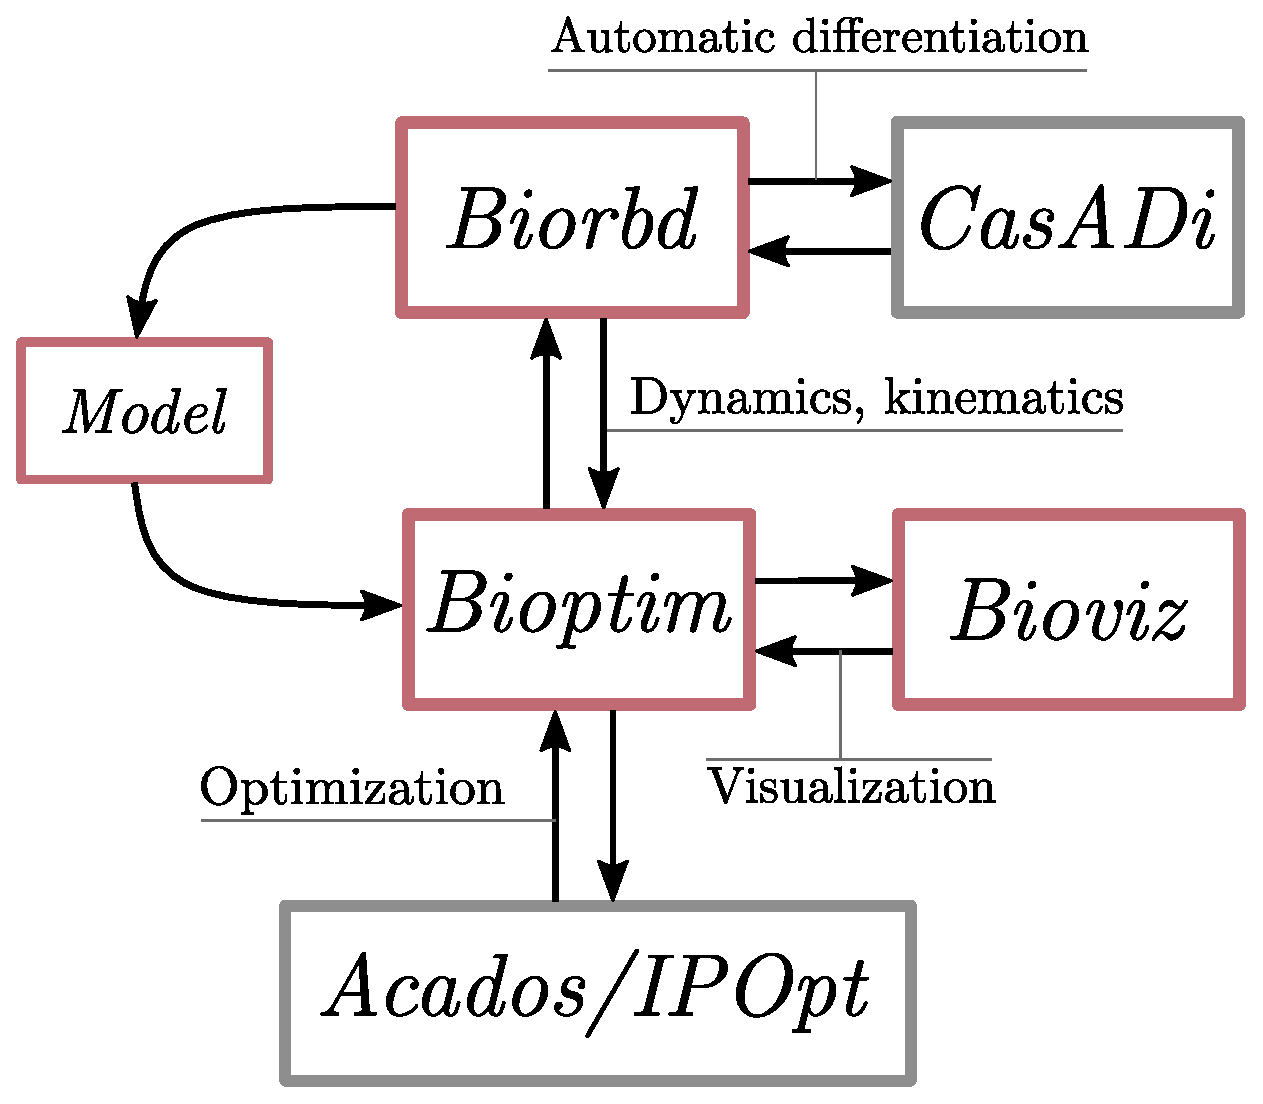
\includegraphics[width=0.9\columnwidth]{figures/dependencies.eps}
\caption{\bioptim dependencies flowchart. The red-boxed software are developed by the S2M team. The \bioptim part is further detailed in Fig.~\ref{fig:flowchart}.}
\label{fig:dependencies}
\vspace*{-0.8cm}
\end{figure}

Concerning the non-linear solver, a variety of software exist and have been used to solve transcribed musculoskeletal NLPs.
They can use different heuristics: interior point methods (\ipopt, \cite{wachter2006implementation}) or sequential quadratic programming (\textit{snopt} \cite{gill2005snopt}, \acados \cite{verschueren2018towards}), but they are all gradient based.
Therefore, derivatives of the NLP cost function and constraints are required to perform optimization.
These derivatives can be obtained by finite differences (often implemented but inaccurate thus comprising convergence) or computed exactly using automatic differentiation (requiring to write all dependencies of the software in symbolic variables), using, e.g., \casadi \cite{andersson2019casadi}.

In order to promote the use of musculoskeletal optimal control among biomechanics researcher, we identified a strong need for a dedicated tool, as shown by the recently launched \moco \cite{dembia2020opensim}. 
The biomechanics community being mainly composed of software users, such a tool should request a flexible user interface written in a widely used high-level and if possible open-source language (e.g. Python) with a low-level core (e.g. C++) for efficiency. 

To develop such a software, four interrelated components are essential in our opinion: \textit{i)} a musculoskeletal modeling software, with a visualization module (multibody kinematics and dynamics, muscle dynamics, etc.), \textit{ii)} a method for automatic differentiation, \textit{iii)} a discretization approach, and \textit{iv)} one or several nonlinear programming (NLP) solvers. 
General-purpose optimal control software (e.g. \gpopsii \cite{patterson2014gpops}, \muscodii \cite{leineweber2003efficient1,leineweber2003efficient2}, \acado \cite{houska2011acado}]) address \textit{ii)} to \textit{iv)} but they need to be interfaced with a musculoskeletal modeling module and they do not provide any built-in biomechanics features (physiological cost functions, kinematic constraints, etc.). 
In that sense, the aforementioned \moco, is a welcome initiative that draws its strength from its integration with the widely used \opensim.
However, it faces the following limitations: it uses finite differences to avoid the complexity of adapting the \opensim codebase to support automatic differentiation, it uses direct collocation as transcription method, preventing the use of adaptive ODE solvers and it is not as flexible as required by the community, since it requires the user to develop new features, such as new objective functions, in C++. 

The objective of the present paper is to introduce \bioptim\footnote{\url{https://github.com/pyomeca/bioptim}\\\comment{DOI: 10.5281/zenodo.4562883}{J'ai aussi mis la citation après, mais on peut la retirer..}}~\cite{bioptim2021michaud}, an \comment{open-source}{je l'ai corrigé quelques fois, mais ça semble revenir, open source ne prend pas de tiret} optimal control software dedicated to musculoskeletal biomechanics.
\bioptim is based on C++ code for computational efficiency but the user interface is written in Python for flexibility and ease-of-use. 
The OCP transcription uses direct multiple shooting to preserve the possibility of using arbitrarily accurate ODE solvers for the integration, which is fully parallelized for more efficiency.
\bioptim's core is fully written in \casadi symbolics to benefit from algorithmic differentiation and to exploit \casadi 's interface with several non-linear solvers (\ipopt, \snopt).
Moreover, \bioptim is interfaced with the cutting-edge solver \acados, a recent NLP solver dedicated to direct multiple shooting, intended for real-time applications.
The purpose of \bioptim is to allow fast and flexible musculoskeletal OCP formulation and solving by providing a framework with a lot of typical biomechanics problem already implemented and customizable.

The paper is organized as follows: first, the design and implementation of \bioptim are described.
Next, the versatility and performances of \bioptim are shown through a variety of examples available online. 


\section{Implementation and Design}\label{sec:design&impl}
\subsection{Implementation and dependencies}
\bioptim is the top layer of a succession of software on which it depends to perform various calculations (\textit{Biorbd}: dynamics and MSK modeling; \textit{CasADi}: automatic differentiation; \textit{IPOpt, Acados}: optimization; \textit{Bioviz}: visualization).
Within this software bundle, \bioptim 's main role is to shape the problem in order to allow its dependencies to communicate efficiently, while providing an intuitive and flexible interface to the user (Fig.~\ref{fig:dependencies}).
Therefore, it was chosen to be written in Python for its flexibility and its widespread use among researchers.
However, all intensive calculations behind the interface are performed in C or C++, keeping \bioptim both fast and easy to customize.

\begin{figure}[t!]
\centering
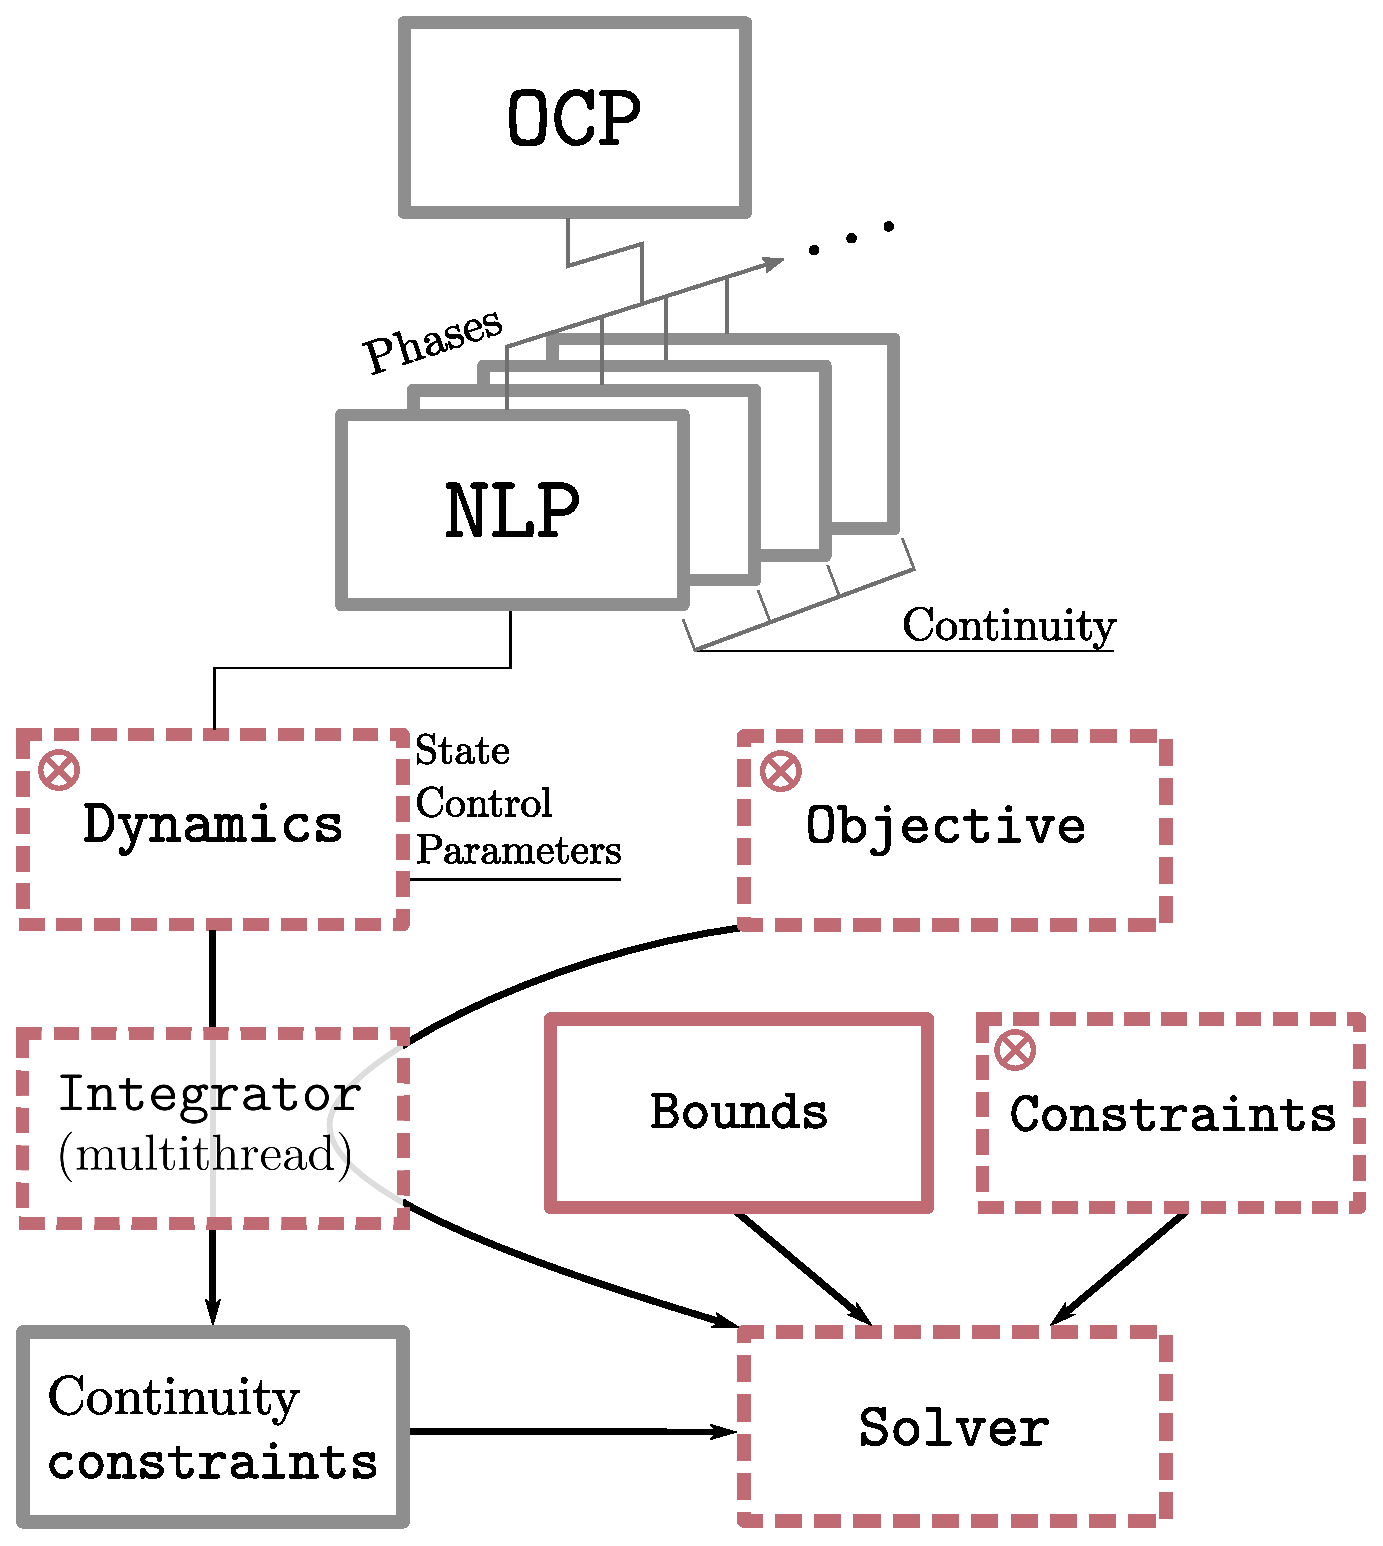
\includegraphics[width=0.9\columnwidth]{figures/design.eps}
\caption{\bioptim design flowchart.}
\label{fig:dependencies}
\vspace*{-0.5cm}
\end{figure}


\subsection{Design}
\bioptim shapes and solves optimal control problems whose two required entries are a model (.\textit{bioMod} file) and an OCP.
The model file contains the geometrical characteristics, the segment inertias, the geometrical markers, the actuators of the model (muscles and joint torques accounting for angle/angular velocity/torque relationships) as well as bounds on joint kinematics and torques. 
It also allows the user to design or import meshes for visualization purposes.
The OCP is implemented as a combination of nonlinear problems (NLPs) for allowing the formulation of multi-staged OCPs. Each NLP has the following attributes: a dynamics type, an objective function, constraints, a number of shooting points, the duration of the problem and initial guesses.
Based on these inputs, \bioptim properly sets up the multiple shooting transcription of the OCP, with appropriate continuity constraints in the case of multiple NLPs, and shapes it up to feed the chosen non-linear solver (Ipopt or Acados). 

\subsubsection{Dynamics types}
The dynamics type defines which variables are states ($\state$), which ones are controls ($\control$) and which ones are parameters ($\param$).
Then, it implements the ordinary differential equation governing the state transition:

\[
\dstate = f(\state, \control, \param).
\addtag
\label{eq:state_transition}
\]

\noindent More than 10 dynamics are implemented in \bioptim \footnote{\href{https://github.com/pyomeca/bioptim/blob/master/bioptim/dynamics/dynamics_functions.py}{github link}}, among which the controls can be muscle excitations/muscle activations/joint torques, the states can be joint kinematics/muscle activations, including/excluding contacts, etc.
Even if these dynamics types exhaustively span the current usages in biomechanics, a custom dynamics type is also pre-implemented to allow easy problem customization.

\subsubsection{Objective functions}
Accordingly to the optimal control formalism, there are two main types of objective functions, namely Lagrange and Mayer. Lagrange types are running objectives, integrated over the NLP duration. Mayer types are time-specific objectives. Classically, they correspond to a terminal objective, but to be more versatile, they can be defined at any instant in \bioptim.

These objective functions can depend on any of the optimization variable, \textit{i.e.} the controls, the states, the parameters and the duration of the problem. A lot of objective function types are already implemented in \bioptim ($>\!20$), among which tracking/minimizing, on the states/controls/markers/contact forces/problem duration, etc. Should one go missing, a custom objective type is also pre-implemented.

When declaring the desired list of objective function for a given NLP, each objective function type is associated with a weight, and the user can flexibly choose on which components of the vector variables the objective must apply. If applicable (for tracking objective functions mainly), the user must also specify the numerical target of the objective.

\subsubsection{Constraints}

\section{Examples}\label{sec:Examples}
In this section, six applications are presented to illustrate the versatility of \bioptim and give a practical overview on how to use its main features.
The settings and performances (convergence time, single shooting integration error, optimized objective) of each OCP are summarized in Tab.~\ref{tab:Perfs_and_detailed_implementations_of_each_example}. 
When possible, problems were solved with both \ipopt and \acados.
In the following, bold symbols denote vectors and starred ones denote reference or tracked quantities.


\subsection{Muscle activation driven pointing task}\label{ex:poiting}
%
\begin{figure}[t!]
\centering
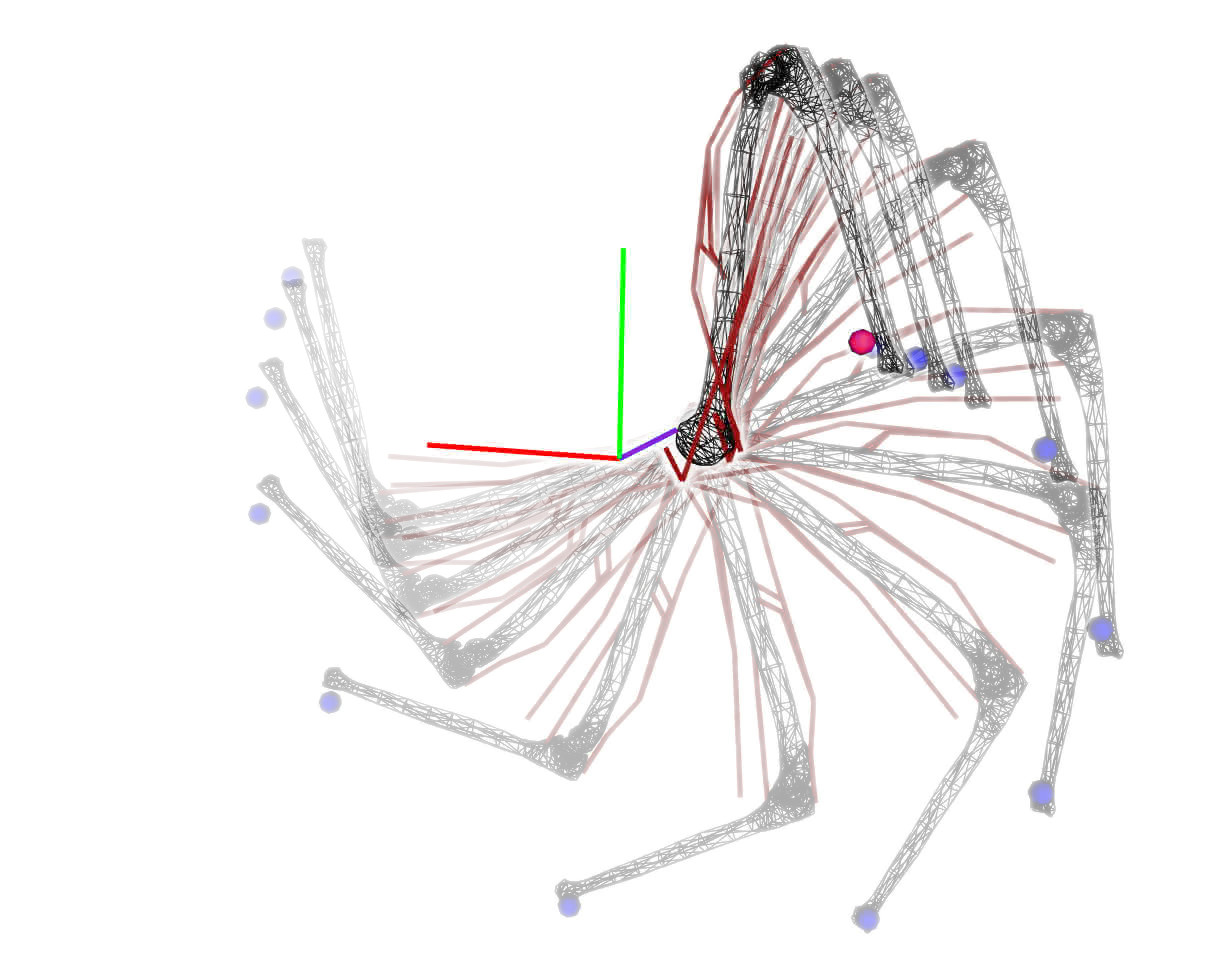
\includegraphics[width=\columnwidth]{figures/activation_pointing.jpeg}\\
\caption{Snapshots of an optimized activation-driven pointing task with \acados. The arm starts facing upwards in left hand part of the picture and ends facing downwards in the right hand part. The marker fized on the Ulna is depicted in blue and the scene-fixed target marker is depicted in red. Red lines show the lines of actions of the muscles.}
\label{fig:snapshots_activation_driven_pointing}
\end{figure}
\begin{figure*}[t!]
\centering
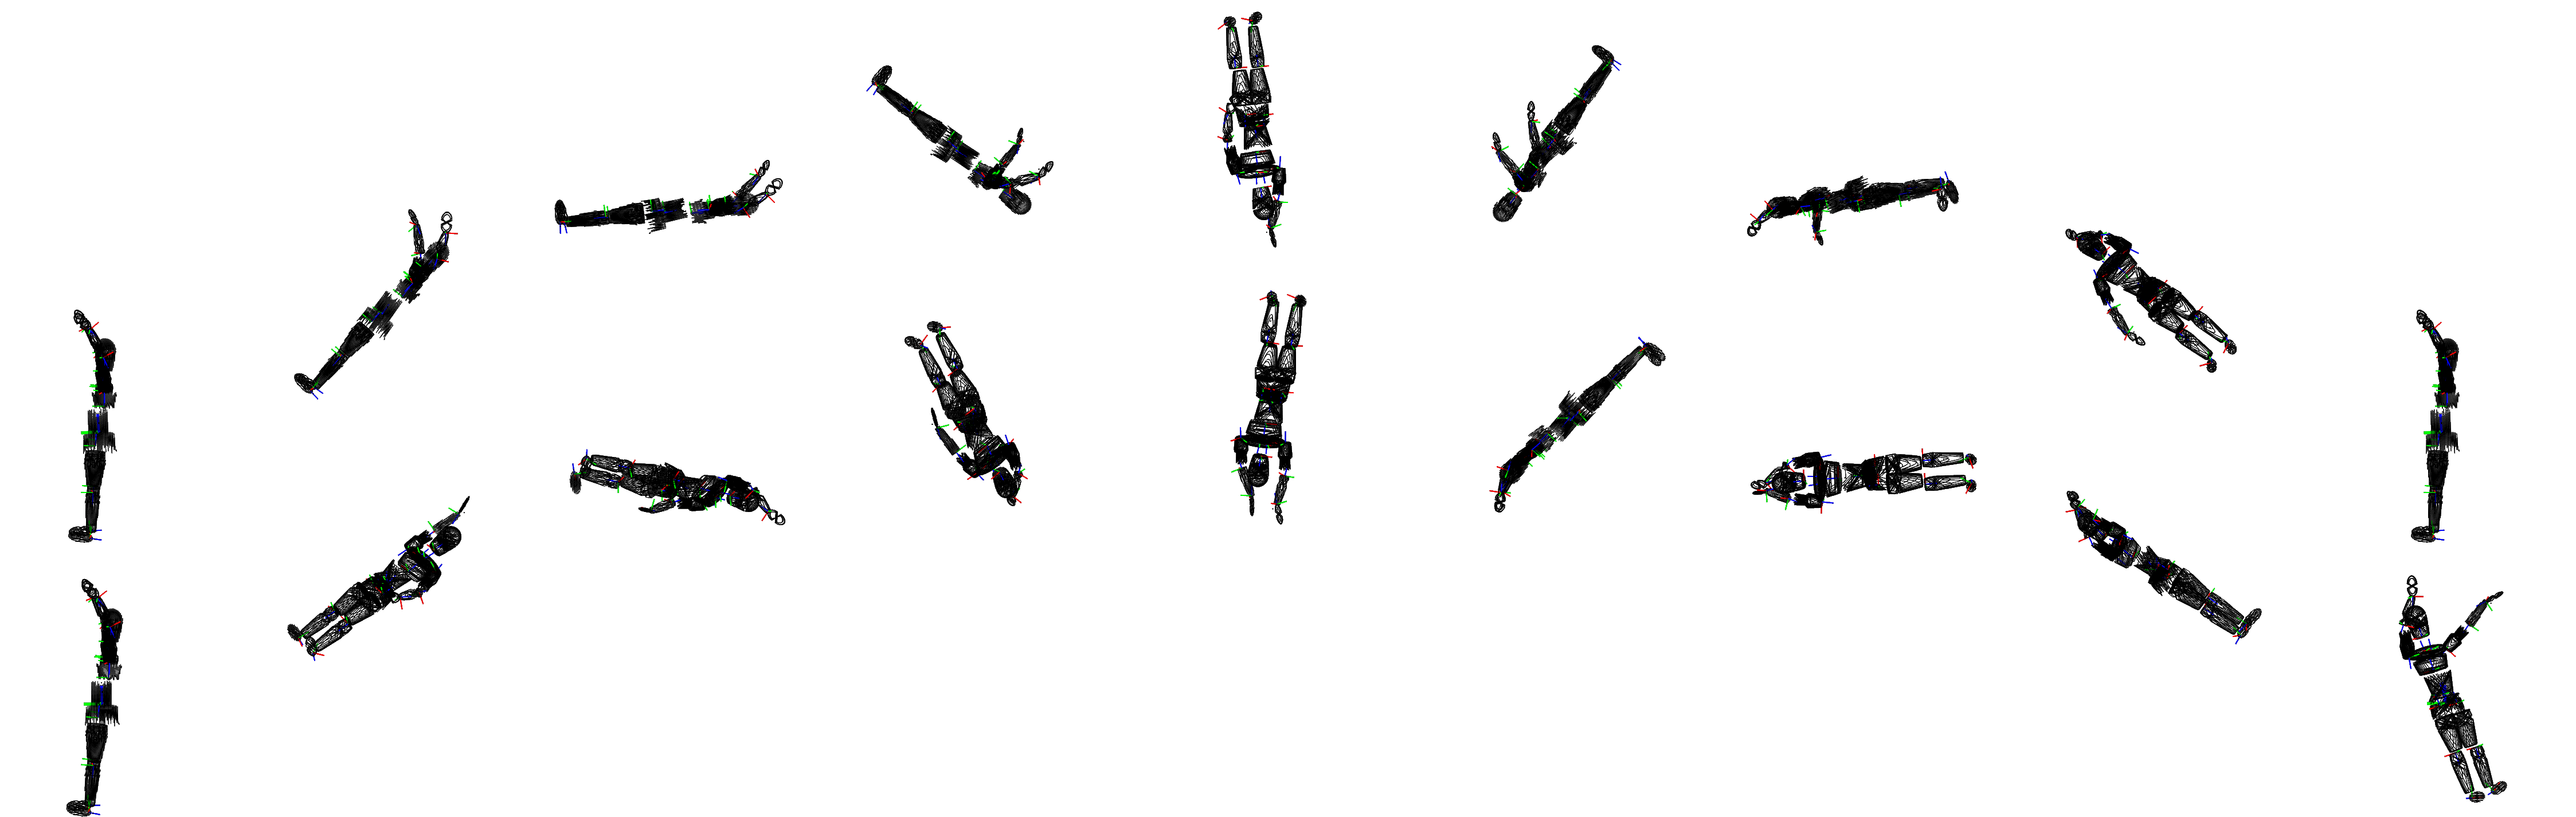
\includegraphics[width=\textwidth]{figures/Both_Bioptim_MaxVrille.png}
\caption{Snapshots of maximally twisting somersaults driven by shoulder torque actuators and a free base whose rotation is either expressed by Euler angles (top) or by quaternions (bottom).}
\label{fig:snapshots_quaternion_base_twisting_somersault}
\end{figure*}
%
In this first example, the goal was to achieve a muscle activation driven pointing task using a 2-DoF arm model with 6 muscle elements. 
In addition to muscle-induced torques, pure joint torques were added to compensate for the model weaknesses.
The main term (highest weight) of the objective function (Eq.~\ref{eq:cost_pointing}) is a Mayer objective, corresponding to the pointing tasks at the final node, to superimpose two markers, the first one, $\mathbf{m_u}$, fixed in the Ulna system of coordinates and the second one, $\mathbf{m^*_s}$, fixed in the scene.
The three Lagrange terms  were added for control regularization (muscle activation $\bf{a}$ and joint torques $\boldsymbol{\tau}$) and for state ($\bf{x}$) regularization:
\[
\begin{aligned}
	\mathcal{C} = 	&~\omega_1~\underbrace{\|\mathbf{m_u}(T)-\mathbf{m^*_s}\|^2}_{\mathtt{TRACK\_MARKERS}}~\\
	&\int_{t=0}^T\underbrace{\|\bf{a}\|^2}_{\mathtt{MIN\_ACTIVATION}}~
	+\underbrace{\|\boldsymbol\tau\|^2}_{\mathtt{MIN\_TORQUE}}~
	+\underbrace{\|\bf{x}\|^2}_{\mathtt{MIN\_STATE}}~ dt,
\end{aligned}
\addtag
\label{eq:cost_pointing}
\]

\noindent where T is the duration of the motion, and $\omega_1=1e5$.
The movement lasted for 2~seconds and was discretized using 50~shooting nodes with a 5-steps RK4 integration in-between.
The problem was solved using \ipopt (with exact Hessian computations) and \acados (with a Gauss-Newton approximation of the Hessian) resulting in two very close solutions.
\acados was about 50 times faster than \ipopt and was better at enforcing the continuity constraints (as shown by the single shooting error in Tab.~\ref{tab:Perfs_and_detailed_implementations_of_each_example}).
\ipopt however ended up with a smaller optimized objective (20.8 \textit{vs} 23.2), leading to a more optimal solution than \acados. 
Superimposed snapshots of the optimal motion found with \acados are displayed in Fig.~\ref{fig:snapshots_activation_driven_pointing}.
It is worth mentioning that for the purpose of this illustration, no constraint was given on the shoulder range of motion to ensure physiological muscle trajectories. 










\subsection{Quaternion base twisting somersault}\label{ex:somersault}
The goal was to maximize the twist rotation ($\phi$) in a backward somersault.
The model is composed of a 6-DoF root segment and two 1-DoF torque actuated arms.
The OCP was solved for two models.
First, rotations of the root segment were expressed as Euler angles.
They were expressed as a quaternion for the second model.
The objective functions were written as follow:

\begin{eqnarray}\label{eq:ocp_Trampo}
\mathcal{J} = -\underbrace{\int_0^T \dot{\phi}~dt}_{MINIMIZE\_TWIST}  +~\omega_1 \underbrace{\int_0^T \sum_{i=1}^{2}~\tau_{i}^2~dt}_{MINIMIZE\_ TORQUE},
\end{eqnarray}
with $\omega_1 = 1\times 10^{-6}$, T the duration of the movement and $\tau_{i}$ the torque control of the $i^{th}$ arm DoF.
The first term of the objective function (Eq.~\ref{eq:ocp_Trampo}) corresponds to maximizing the twist velocity and the second term is for control regularization.


The movement lasted for approximately 1 second and was discretized in 100 shooting nodes.
The solutions for both models were similar (Fig.~\ref{snapshots_quaternion_base_twisting_somersault}) highlighting the equivalence of the two rotation representations.
Euler angles have the advantage to be easily interpretable, but they suffer from the loss of a DoF at the gimbal lock.
The use of quaternion representation is advantageous for numerical stability when a joint is free to rotate on a wide three-dimensional range for motion.


\begin{figure*}[t!]
\centering
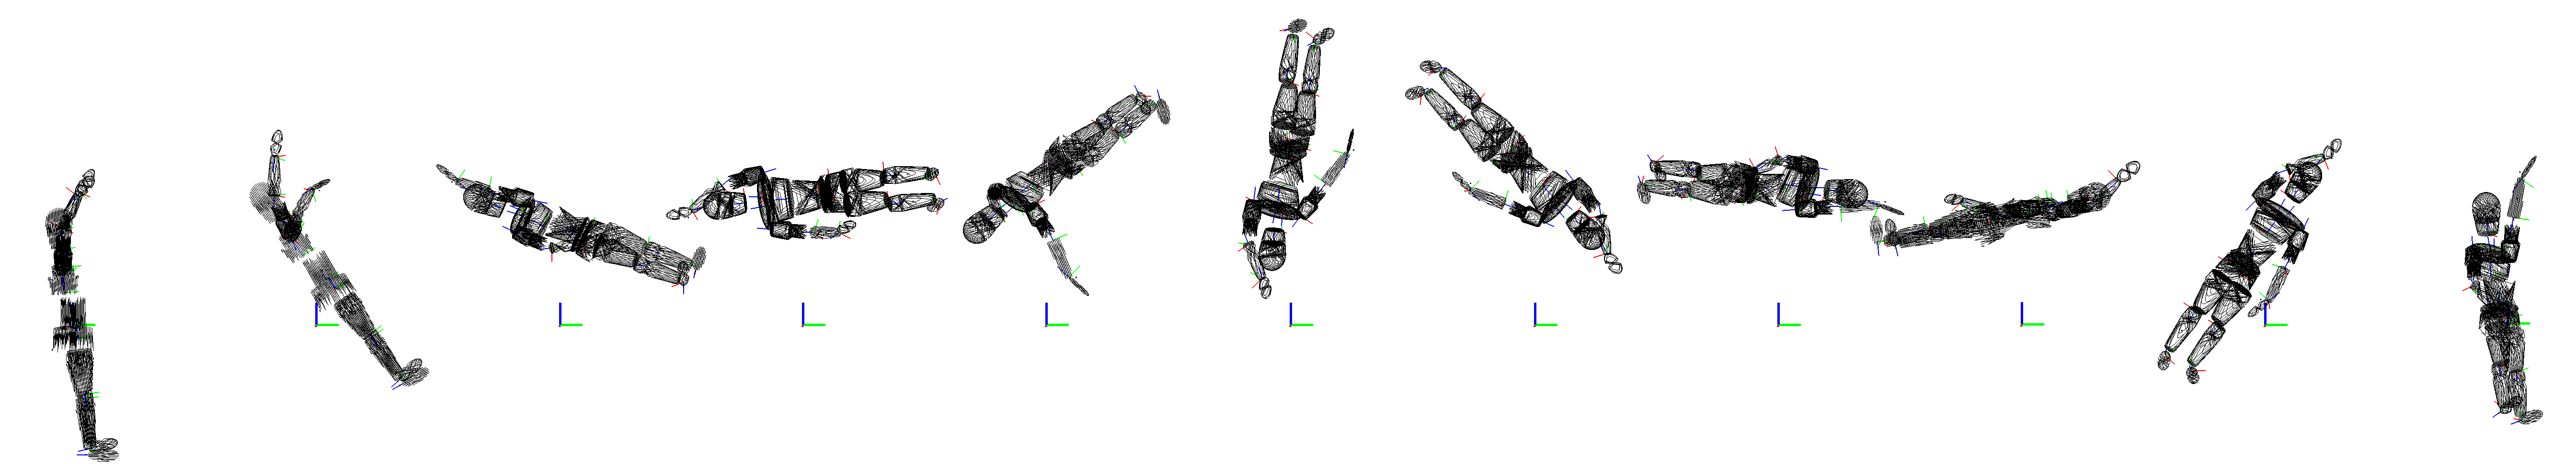
\includegraphics[width=\textwidth]{figures/Euler_Bioptim_MaxVrille_2.png}\\
\vspace*{0.5em}
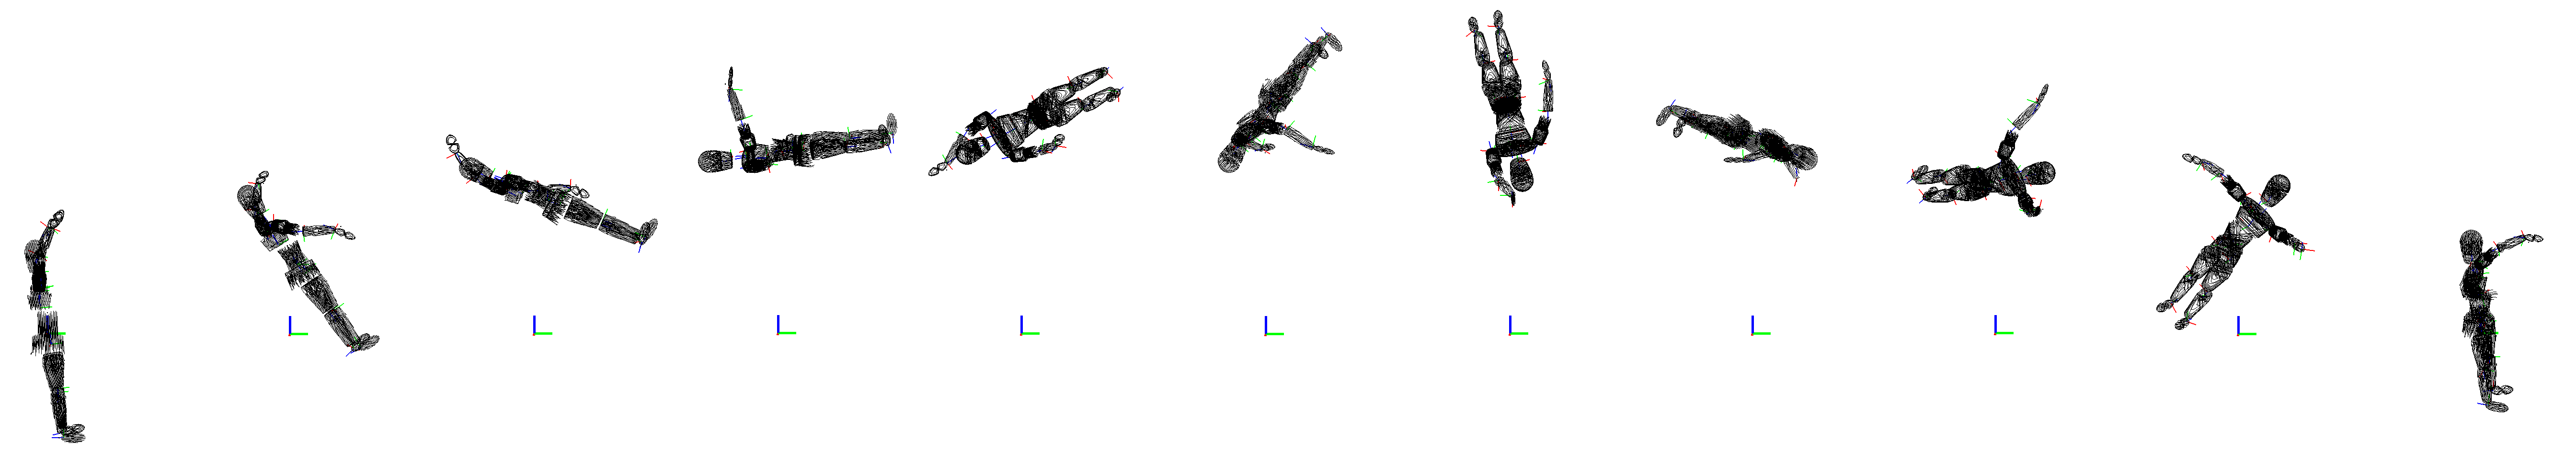
\includegraphics[width=\textwidth]{figures/Quat_Bioptim_MaxVrille_2.png}
\caption{Snapshots of a maximally twisting somersault driven by shoulder torque actuators and a free base expressed by Euler angles (top) or quaternions (bottom).}
\label{fig:snapshots_quaternion_base_twisting_somersault}
\end{figure*}


% \begin{table}[h!]
% \caption{\small Objective terms of quaternion base maximally twisting somersault}
% \label{tab:Quaternion_base_twisting_somersault}
% \centering
% \begin{tabular}{c c c c}
% \toprule 
% & Type & Function & Weight \\ 
% \midrule
% $\#1$ & Lagrange & MINIMIZE\_TWIST & $-1e1$ \\ 
% \midrule
% $\#2$ & Lagrange & MINIMIZE\_ TORQUE & $1e-6$ \\ 
% \bottomrule
% \end{tabular}
% \end{table}















\subsection{Pendulum on a spring}\label{ex:spring}
This spring-mass-pendulum-based example is presented to introduce \textit{bioptim}'s ability to use of external forces.
The goal was to maintain the position of a $\SI{1}{kg}$ mass hanging on a linear spring attached to the ground.
A $\SI{0.2}{m}$-long pendulum weighting $\SI{10}{kg}$ was attached to the mass and free to rotate in one dimension (Fig.~\ref{fig:Mass_Pendulum_Model}).
In addition to the spring force, the mass was actuated by a vertical force (e.g., somebody pulling on it) while the pendulum rotation was passive.
The system therefore comprised two DoFs, the mass position ($q_m$) and the pendulum angle ($q_p$) and one control input, the vertical force pulling on the mass ($f$). 
\begin{figure}[h!]
\centering
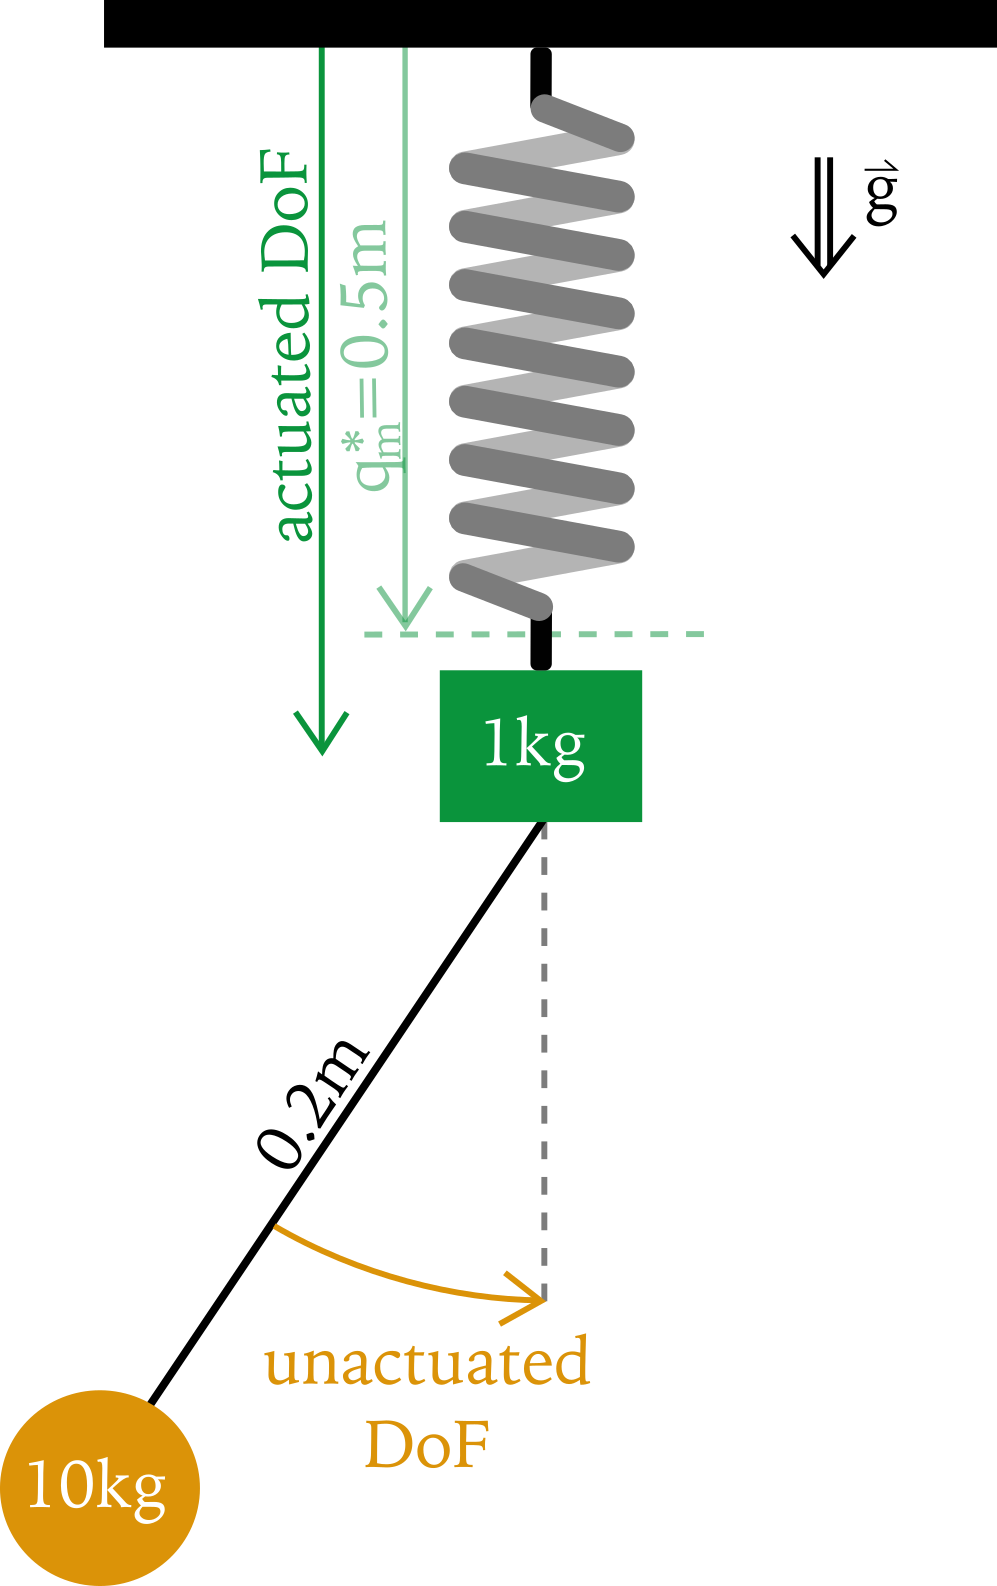
\includegraphics[width=0.35\columnwidth]{figures/Mass_Pendulum_Model.png}
\caption{Definition of the spring-mass-pendulum model.}
\label{fig:Mass_Pendulum_Model}
\end{figure}
The spring force $f_s$ was:
\[
\begin{aligned}
f_s = -k*q_m,
\end{aligned}
\addtag
\label{eq:f_ext}
\]
with k the spring stiffness constant.\\
The OCP was composed of two phases each lasting for $\SI{5}{s}$, with 50 shooting nodes.
In the first phase, no objective function was minimized and $f$ was constrained to $0$ letting the mass oscillating freely. 
Then, in the second phase, a cost function (Eq.\ref{eq:ocp_Pendulum}) was minimized, to enforce a specific position for the mass.
Theis objective function, exclusively composed of Lagrange terms, was formulated as follow:
\[
\mathcal{J} = \underbrace{\int_{T/2}^T (q_m - q_m^*)^2~dt}_{\mathtt{TRACK\_STATE}}  +~\omega_1 \underbrace{\int_{T/2}^T ~\tau^2~dt}_{\mathtt{MIN\_ TORQUE}},
\addtag
\label{eq:ocp_Pendulum}
\]

\noindent with $q_m$ and $q_m^* = -0.5m$ respectively the optimized and reference positions of the mass, $\omega_1 = 1\times 10^{-6}$, T the duration of the movement and $\tau$ the force control of the mass.
The first term of the objective function (Eq.~\ref{eq:ocp_Pendulum}) acts as a position controller for the mass.
The second as added for control regularization.


During the first phase, the mass is oscillating passively around it's stationary position due to the force exerted by the spring.
However, when the mass gain the ability to react actively with force actuation, it stabilizes around the targeted position (Fig.~\ref{fig:Mass_Pendulum_Fext_graphs}).
This example highlights the possibility of using optimal control to find activation patterns compensating for external passive forces (e.g., ortheses flexibility, contact surface deformation, interaction between two models, ...).

\begin{figure*}[t!]
\centering
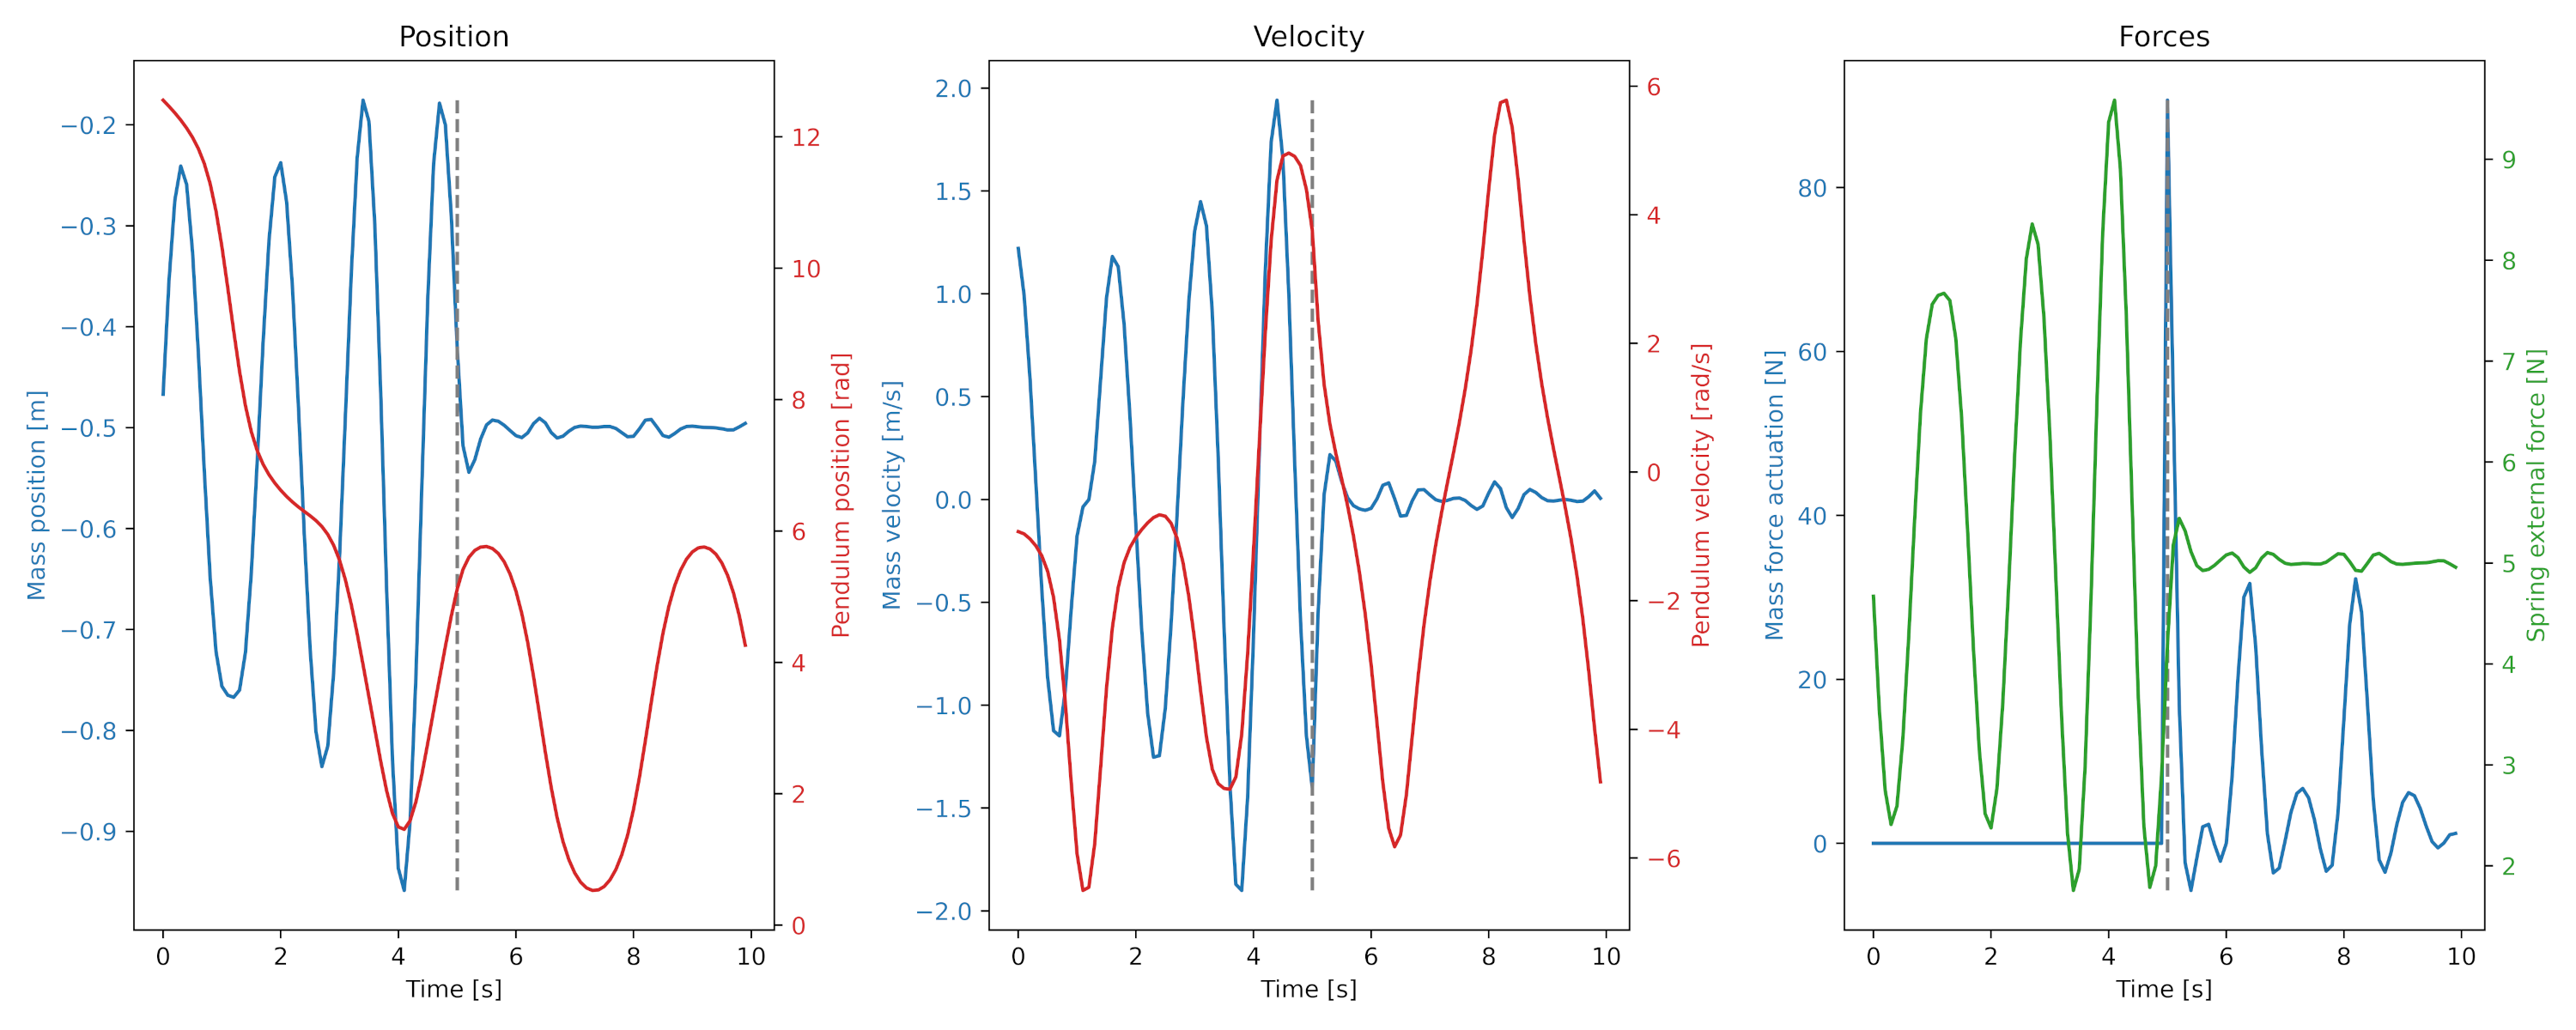
\includegraphics[width=\textwidth]{figures/Mass_Pendulum_Fext.png}
\caption{Optimal kinematics of the mass-pendulum-spring system. Gray dashed lines show the stage transition, blue lines are related to the mass, red lines are related to the pendulum and the green line is related to the spring.}
\label{fig:Mass_Pendulum_Fext_graphs}
\end{figure*}
















\subsection{Multiphase torque driven walking cycle}\label{ex:walking}
This example is presented to introduce \textit{bioptim}'s ability to deal with a multiphase locomotion estimation problem with muscle actuation and contact forces.
The goal was to estimate muscles activation by tracking markers trajectories and ground reaction forces and moments. 
The model was a 3D leg with 12 DoFs (6-DoFs pelvis, 3-DoFs hip, 1-DoF knee and 2-DoFs ankle), driven by 17 muscle activations and residual joint torques to compensate for potential muscle actuation weaknesses. 
The gait cycle was defined from the first heel strike to the end of the swing phase discretized into 90 shooting intervals. 
To follow the natural rolling of the foot, the stance was divided into three phases (heel, flatfoot and forefoot contacts) of fixed duration deduced from experimental force platform data and markers position ($0.05$, $0.36$ and $0.16$\:s).
The swing phase lasted $0.38$\:s. 
The interaction between the ground and the foot was modeled using a 4-contact points model located at the heel and the forefoot (first, fifth metatarsi and hallux).
The optimization problem consisted in minimizing the errors between predicted $\bf{m}$ and reference $\bf{m}^*$ markers trajectories, predicted $\bm{\mathcal{F}}$, $\bm{\mathcal{M}}$ and reference $\bm{\mathcal{F}^*}$, $\bm{\mathcal{M}}^*$, respectively ground reaction forces and moments at all contact points.
$^*$ stands for reference (i.e., measured) data.
A regularization term on muscle activations, $\bf{a}$, was also added (least-activations) as well as a penalization term on the residual torques $\boldsymbol{\tau}$:

\[ 
\resizebox{0.9\columnwidth}{!}{$ 
\begin{aligned}
%\mathcal{J} = &\int_{t=0}^{T}\underbrace{\omega_1(\|m_p - m_m\|^{2})}_{\mathtt{TRACK\_MARKERS}}~ 
%+ ~ \underbrace{\omega_2(\|f_p - f_c\|^{2})}_{\mathtt{TRACK\_FORCES}}\\
%&+ ~ \underbrace{\omega_3(\|tau^f_p - tau^f_m\|^{2})}_{\mathtt{TRACK\_MOMENTS}}~
\mathcal{J} = &\int_{t=0}^{T}\underbrace{\omega_1(\|\bm{m} - \bm{m}^*\|^{2})}_{\mathtt{TRACK\_MARKERS}}~ 
+ ~ \underbrace{\omega_2(\|\bm{\mathcal{F}} - \bm{\mathcal{F}}^*\|^{2})}_{\mathtt{TRACK\_FORCES}}\\
&+ ~ \underbrace{\omega_3(\|\bm{\mathcal{M}} - \bm{\mathcal{M}}^*\|^{2})}_{\mathtt{TRACK\_MOMENTS}}~
+ ~ \underbrace{\omega_4\|\bf{a}\|^2}_{\mathtt{MIN\_ACTIVATION}}
+ ~ \underbrace{\|\boldsymbol{\tau}\|^2}_{\mathtt{MIN\_TORQUE}}~dt, 
\end{aligned}  
$}  
\addtag  
\label{eq:ocp_walk}  
\]

\noindent where $\omega_1$=1e5, $\omega_2$=0.1, $\omega_3$=0.1, $\omega_4$=10 are  weighting factors and $T$ is the the duration of the current phase.\\

Non-slipping ($\mathtt{NON\_SLIPPING}$) and unilateral contact force ($\mathtt{CONTACT\_FORCE}$) constraints were added to prevent the foot from slipping and pulling from the ground. 
In between phases, the use of the $\mathtt{IMPACT}$ state transition allowed to represent the gain or loss of contact(s) in the dynamics (e.g., swing phase to heel strike [Felis (2016)]) \\
% ~\cite{felis_2016_contact}[Felis (2016). Synthesis of Full-Body 3-D Human Gait using Optimal Control Methods. doi:10.1109/ICRA.2016.7487294]

Tracking experimental data allowed to reproduce leg motion during the walking cycle (Fig.~\ref{fig:snapshots_multiphase_walking_cycle}). 
The root mean square tracking error on markers trajectories was $27$ mm (mean error on pelvic and foot markers was $7.5$ mm and $14.7$ mm, respectively). 
Concerning ground reaction forces tracking, the root mean square error was $4.85$ N.
Gluteal muscles were mainly activated during the stance and with a significant activity during the swing phase (Fig.~\ref{fig:muscles_activation_gait} for all activations). 
The Gluteus Maximus was mainly activated during the early flatfoot phase with a maximal activation of $0.2$ allowing to prepare the stance phase. 
For the thigh muscles, the semimembranous, semitendinous and biceps femoris were activated during the early stance phase and terminal swing (maximal activation of $0.3$, $0.4$ and $0.4$, respectively). 
Those results were similar to the characteristic average activity patterns of the lower limb muscles during locomotion described by Winter (1991). 
% ~\cite{winter_1991} [Winter DA (1991). The Biomechanics and Motor Control of Human Gait: Normal, Elderly and Pathological.]
The knee extensors, vastus lateralis, medialis and intermedius followed the same pattern and were mainly activated during the flatfoot phase (ie loading response).
However, the highest activity of the rectus femoris appeared at forefoot phase (terminal stance) and pre swing.
Leg muscles were highly activated (saturation of gastocnemius lateralis and medialis) at the terminal stance and early swing. The tibialis anterior is the sole muscle for dorsiflexion and the only antagonist of the triceps surae in this model which could explain its high activity at the same time. 

\begin{figure*}[t!]
\centering
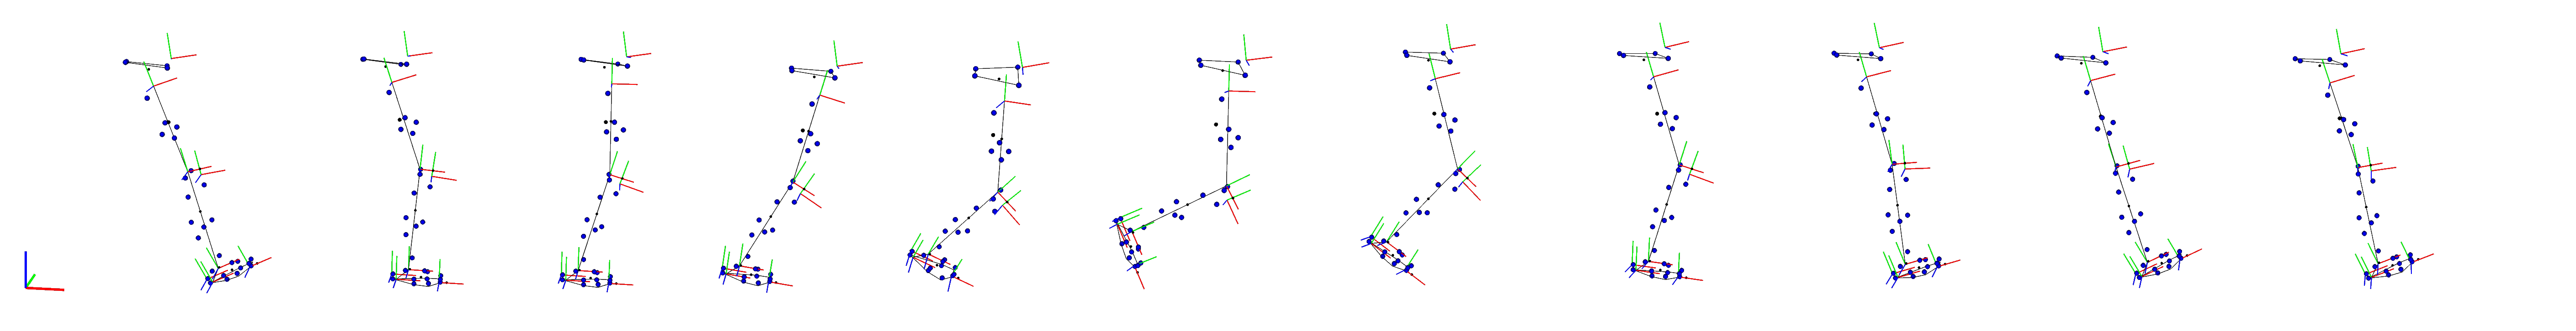
\includegraphics[width=\textwidth]{figures/multiphase_walking_cycle.png}\\
\caption{Snapshots of a walking gait cycle driven by muscles activation.}
\label{fig:snapshots_multiphase_walking_cycle}
\end{figure*}

\begin{figure*}[t!]
\centering
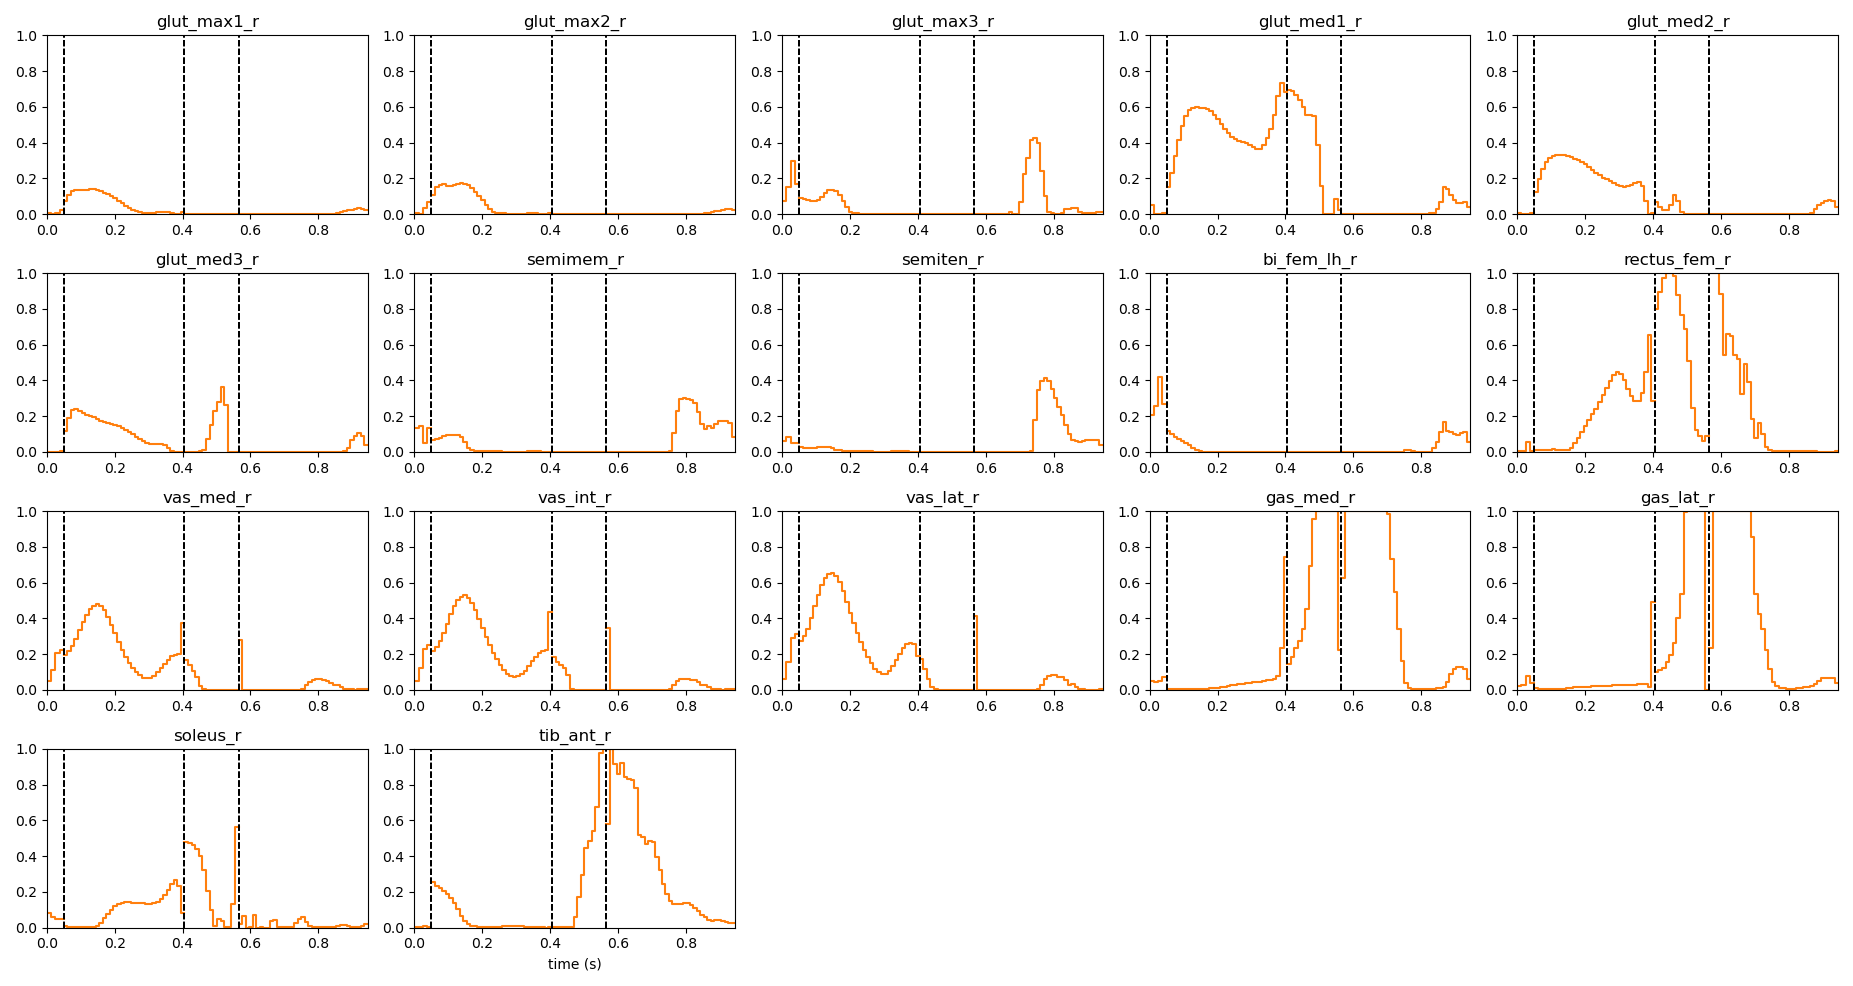
\includegraphics[width=\textwidth]{figures/muscles_control_gait_example.png}\\
\caption{Muscle activity patterns during walking cycle.}
\label{fig:muscles_activation_gait}
\end{figure*}


\subsection{Moving Horizon Estimation of Shoulder Elevation}\label{ex:mhe}
This example is presented to introduce \bioptim's ability to provide real-time estimation of biomechanical variables.
The goal was to perform a real-time estimation of dynamically consistent joint kinematics and muscle forces, using a moving horizon estimation (MHE) approach (i.e. an optimization approach that uses a series of measurements observed over time). 
A shoulder elevation motion was performed with a 4-DoFs ($\bf{q}$) arm actuated by 19 Hill-type muscle elements.
The control inputs of the model were the muscle activations ($\bf{a}$).
The MHE implementation consists in splitting the OCP into a succession of smaller one for processing fixed-size subsets of the tracking data moving forward in time. 
Each time one subproblem is solved, a new measurement is added, the oldest one is discarded and a new subproblem is defined. 
Due to their similarities, the solution of the previous OCP is a good initial guess to the new one. 
The dynamical consistency of the final solution is enforced by continuity constraints on the initial state. 
Each objective function (Eq.~\ref{eq:ocp_exMHE}) was written as the sum of three terms: tracking reference joint angles ($\bf{q^*}$), states and muscle activations regularizations (i.e., least-square criteria): 
\begin{figure}[t!]
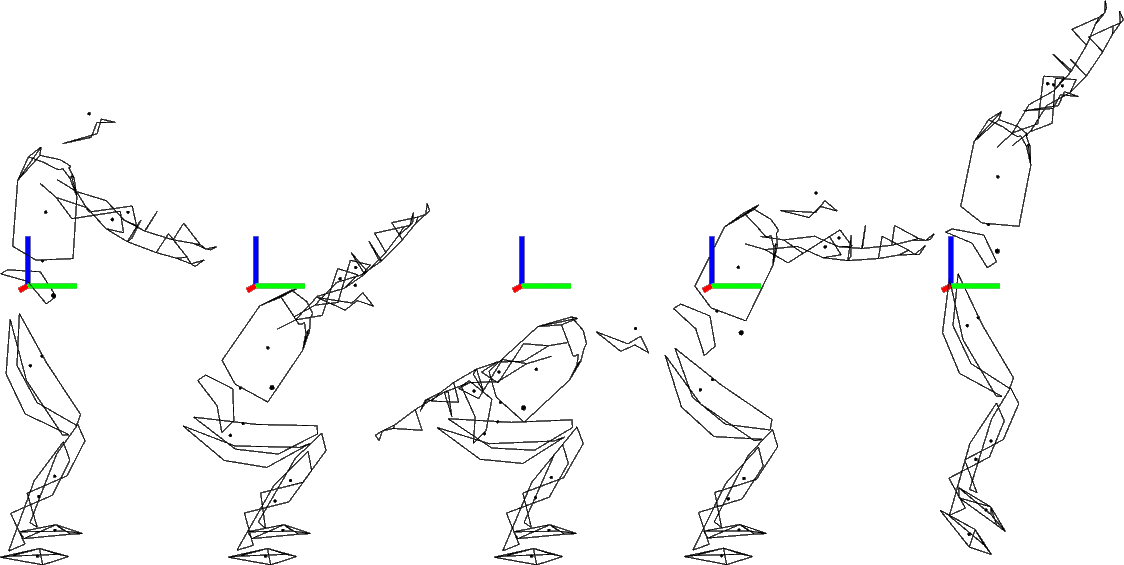
\includegraphics[width=\columnwidth]{figures/kinogramme_jump}
\caption{Snapshots of the push-off phase of a vertical jump (Ex.~\ref{ex:jump}). The avatar reproduces a human-like jump movement. The first four positions represent the first phase of the optimization (i.e., heel and toe in contact with the floor) and the fifth position depicts the end of the second phase (i.e., only the heel in contact with the floor)} 
\label{fig:graph_force_vitesse_longueur}
\end{figure}
\begin{figure*}[t!] 
\centering 
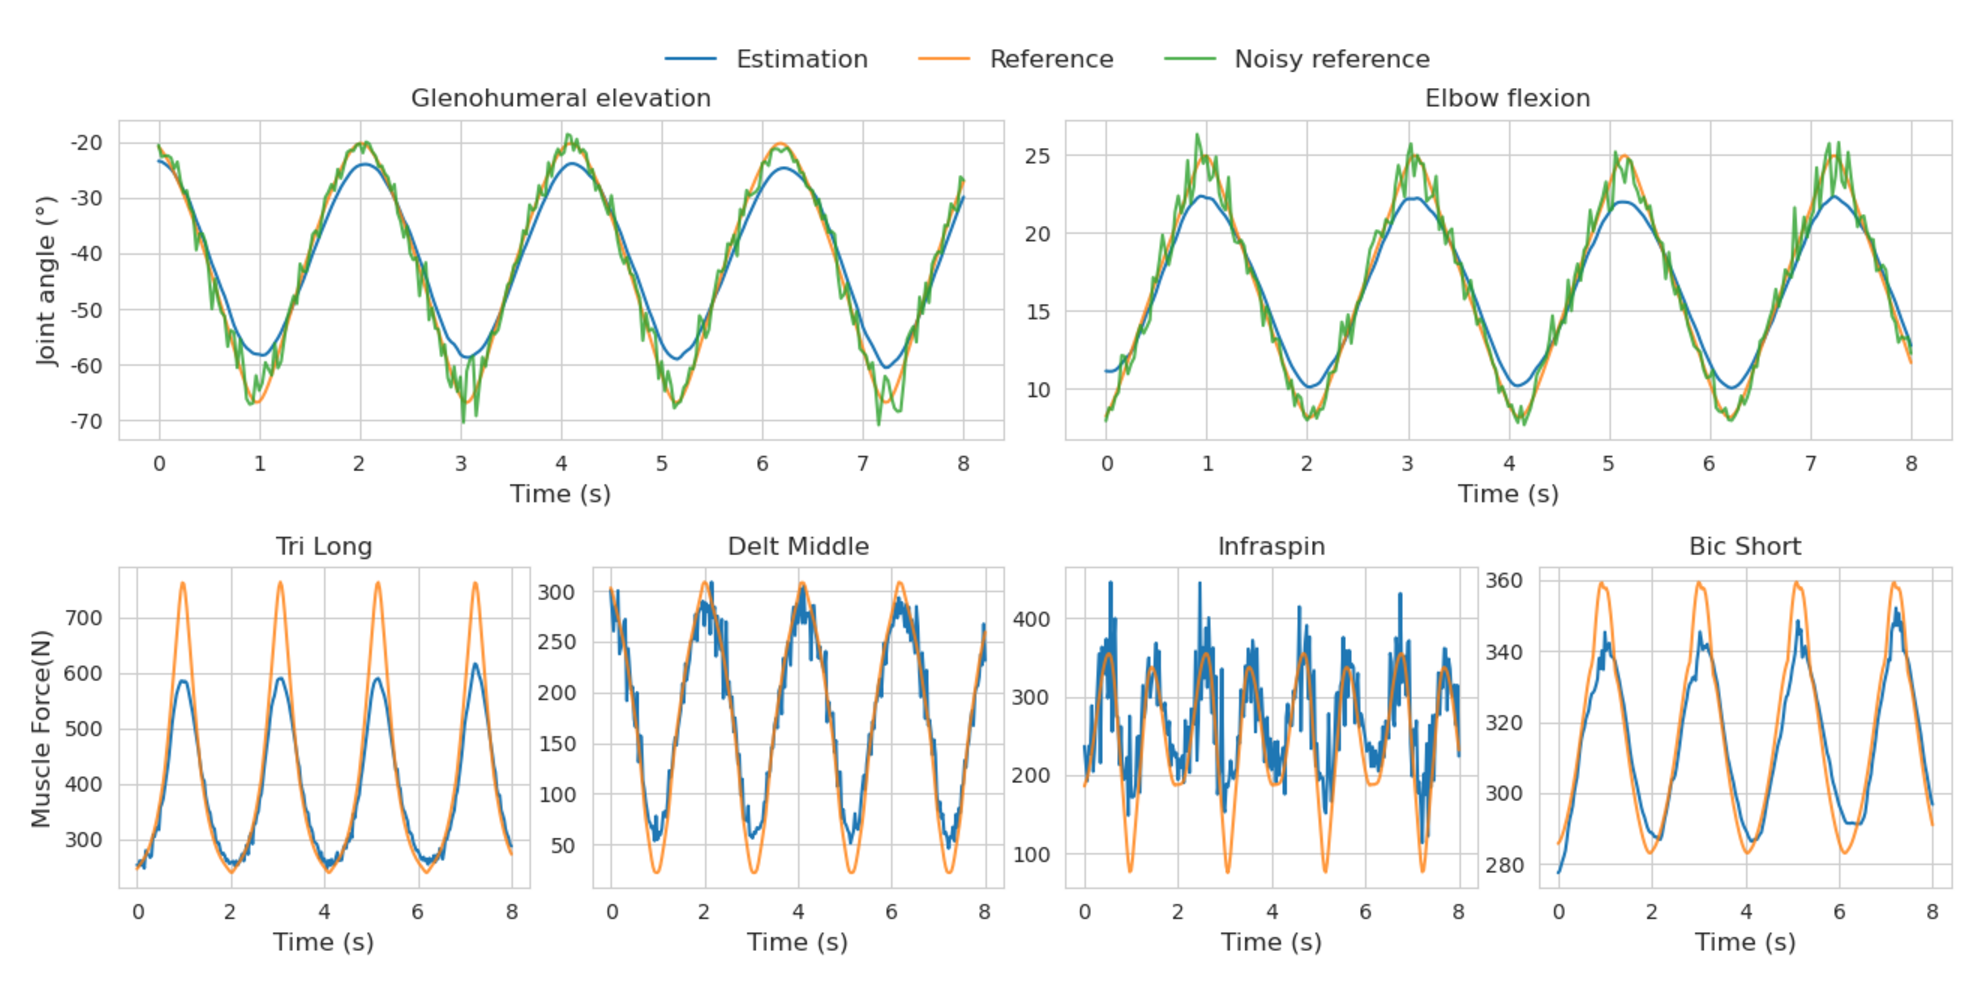
\includegraphics[width=\textwidth]{figures/MHE_results.pdf}\\
\caption{Time series of (1) real-time estimated joint angles (blue), reference joint angle (orange) and noisy reference joint angles (green) of a cyclic motion (up).
(2) Real-time estimated muscle forces (blue) and ground truth muscle forces (orange) of a cyclic motion (bottom) (Ex.~\ref{ex:mhe}).
Only four muscles with significative action (peaks force $>$ 15~N), on the two selected DoFs, are shown.
Muscle abbreviations stand for (from left to right): Triceps Long head, Deltoid Middle, Infraspinatus, Biceps Brachial Short head. (Ex.~\ref{ex:mhe}).} 
\label{fig:MHE_results}
\end{figure*} 
\\ 
\[ 
\resizebox{0.9\columnwidth}{!}{$ 
\begin{aligned}
\mathcal{J} = &\int_t^{t+t_{mhe}}\underbrace{\omega_1´(\|\boldsymbol{q} - \boldsymbol{q^*}\|^{2})}_{\mathtt{TRACK\_STATE}}~ 
+ ~ \underbrace{\omega_2\|\boldsymbol{q\|^2}}_{\mathtt{MIN\_STATE}} 
+ ~ \underbrace{\omega_3\|\boldsymbol{a\|^2}}_{\mathtt{MIN\_ACTIVATION}}~dt, 
\end{aligned}   
$}  
\addtag  
\label{eq:ocp_exMHE}  
\]  

\noindent where $\omega_1 =10^3$, $\omega_2 = 10$, $\omega_3 = 10^2$ and $t_{mhe}$ is duration of each sub-problem. 

In this example, reference data of an $8~s$ series of four arm elevations were generated at 100~Hz, by computer simulation.
A centered Gaussian noise (mean = 0, std = $0.005\:q^*(t)$) was added to $q^*$, to simulate experimental-like joints angle measurements.
Using a windows size of 7 nodes (i.e., 210~ms), the estimator ran at about 33~Hz (one in three reference data frame was sent to the estimator to simulate experimental-like conditions), i.e., two and half times faster than standard biofeedback (13~Hz, \cite{kannape2013self}).
The MHE was able to forecast the movement kinematics with a root mean square error of $1.3\pm0.7^{\circ}$ while providing a realistic estimation of muscle forces close to the ground truth with a root mean square error of $11.1\pm14.9N$ (Fig.~\ref{fig:MHE_results}).



\subsection{Multiphase vertical jumper}\label{ex:jump}
This example was designed to introduce \bioptim's ability to reduce the number of degrees-of-freedom (DoF) of a model via the \texttt{BiMapping} feature, to account for nonlinear boundaries on the controls, and to solve complex multiphase programs.
A total of five phases were used to describe the various dynamics of the jump, namely the push-off phase (i.e., flat foot (two floor contacts\footnote{A contact is defined as a point where forces are applied to cancel its acceleration.}) and then toe only (one contact)), flight (free fall, i.e., no contact) and landing (toe (one contact) and then flat foot (two contacts)).
The transitions between phases where contacts are added are approximated with the build-in inelastic impact \texttt{PhaseTransition.IMPACT}, which computes the velocity of the kinematic chain after an impact.
A pseudo-2D full-body symmetrized model consisting of 3~DoFs at the pelvis (forward and upward translations, tranverse rotation), 1~DoF at the upper limb (shoulder flexion), and 3~DoFs at the lower limb (hip, knee and ankle flexion) was used.
Since this is a full-body model, the root segment (i.e., the pelvis) was left uncontrolled, reducing the number of control variables to 4, namely the shoulder, hip, knee and ankle flexions. 
The objective function with the most important weight was a Mayer objective computed at the end of the push-off phase consisting in maximizing the jump height ($h$) from the free fall equations applied to the center of mass.
The remaining objective functions were regularization terms and terms that favoured a human-like solution. 
\[ 
  \resizebox{0.90\columnwidth}{!}{$ 
  \begin{aligned}
  \mathcal{J} = &~\underbrace{\omega_h~h}_{\mathtt{MIN\_PREDICTED\_COM\_HEIGHT}}~+~\underbrace{\omega_{x} \| \mathbf{\tilde{x}}(T_5) - \mathbf{\tilde{x}}^*\|^2}_{\mathtt{TRACK\_STATE}}\\
  +~&\sum^5_{i=1}~\underbrace{\omega_{t}(T_i - T_{i-1})}_{\mathtt{MIN\_TIME}}~
    +~\sum_{i=2}^4\int_{t=T_i}^{T_{i+1}}\underbrace{\omega_{sd}\left|\left|\frac{d\mathbf{\dot{q}}}{dt}\right|\right|^2}_{\mathtt{MIN\_STATE\_DERIVATIVE}}~dt
  \end{aligned}  
  $} 
  \addtag  
  \label{eq:cost_jumper}
\]
where $T_i$ with $i \in [1, 2, 3, 4, 5]$ are the final times of the i$^{th}$ phase respectively, and $T_0=0$; 
$\omega_h=-100$ is the weight of the jump height term defined negative to maximize it; 
$\omega_t=0.1$, $\omega_{sd}=0.1$ and $\omega_x=1.0$ are the weights of their respective objective functions; 
$\mathbf{\dot{q}}$ is the generalized velocities part of the state vector $\mathbf{x}$; 
and $\mathbf{\tilde{x}}$ is the state vector excluding the translations of the root segment. 
The $\mathbf{\tilde{x}}^*$ corresponds to a reference static position of the avatar with its knee slightly flexed and its arms horizontal.

Joint angles were bounded to human-like limits.
The first node of the first phase was enforced to be equal to $\mathbf{x^*}$ (i.e., including the translations of the root segment to be at the origin). 
Joint velocities were arbitrarily bounded to human-like limits.
Joint torques were bounded with nonlinear torque/angle/velocity relashionships measured on a high-level athlete using an isokinetic dynamometer. 
Non slipping (\texttt{NON\_SLIPPING}) and unilateral (\texttt{CONTACT\_FORCE}) contact force constraints were added to prevent the contact points from slipping and pulling on the ground.
During the ground phases, the heels had to remain over the floor.
To speed-up the solving with \emph{ipopt}, the problem was first solved using a BFGS Hessian approximation for 200 iterations.
Then, starting from this first solution, the problem was re-optimized, with the exact-Hessian computations.

The optimized solution was obtained in 148 iterations of the exact-Hessian optimization \comment{for a total optimization time of $\SI{1780}{\second}$ ($\approx\SI{30}{\minute}$)}{A déplacer dans le tableau}, resulting in a \SI{1.28}{\meter} jump height.
The optimized time for the phases $1$ to $5$ were $0.70, 0.05, 0.99, 0.36, 0.21$ seconds.
The solution reproduced a human proximo-distal strategy (Fig~\ref{fig:jump}), i.e., activating large segments first (for instance the torso) and sequentially adding more distal segments, consequently ending up with the feet.

%
\begin{table*}[h!]
\caption{\small Overview of computational results for the different OCPs cases and links to detailed implementations. The single shooting state trajectory is obtained by forwardly integrating the initial state with the optimized control inputs during 1~second. The single shooting error is computed as the mean RMSE between the optimized state vector and the single shooting one at 1~second.}
\label{tab:Perfs_and_detailed_implementations_of_each_example}
\centering
\begin{tabular}{c l rl rl rl}
\cmidrule[\heavyrulewidth](lr){2-8}
& & \multicolumn{2}{l}{\ref{ex:poiting} Activation-driven pointing} & \multicolumn{2}{l}{Ex\# 2} & \multicolumn{2}{l}{Ex\# 3} \\
\cmidrule[\heavyrulewidth](lr){3-4}
\cmidrule[\heavyrulewidth](lr){5-6}
\cmidrule[\heavyrulewidth](lr){7-8}

\mymultirow{4}{Setup} & \# states $\xt$            & \multicolumn{2}{c}{4}  & --    & --     & --    & --\\
                      & \# control $\ut$           & \multicolumn{2}{c}{6}  & --    & --     & --    & --\\
                      & \# shooting nodes          & \multicolumn{2}{c}{50} & --    & --     & --    & --\\
                      & OCP duration (s)           & \multicolumn{2}{c}{2}  & --    & --     & --    & --\\
                      &                            & \ipopt  & \acados        & \ipopt  & \acados  & \ipopt  & \acados \\
\mymultirow{3}{Solve} & \# NLP iterations          & 47     & 19            & --    & --     & --    & --\\
                      & Optimized cost             & 20.8 & 23.2        & --    & --     & --    & --\\
                      & Time to convergence (s)    & 22.3    & 0.45          & --    & --     & --    & --\\
                      & Single shooting error    & $<10^{-7}$    & $<10^{-13}$          & --    & --     & --    & --\\
%Example & Link & IPOPT & ACADOS \\ 

%\midrule
%Muscle activation driven pointing task & \href{https://github.com/pyomeca/BiorbdOptim/blob/master/examples/muscle_driven_ocp/static_arm.py}{$\star$} & $10.10$ & $0.2018$  \\ 
%\midrule
%$\bullet$ & $\bullet$ & $\bullet$ & $\bullet$ \\ 
\cmidrule[\heavyrulewidth](lr){2-8}
\end{tabular}
\end{table*}
%









\section{Discussion}\label{sec:discussion}
The purpose of \bioptim is to solve a variety of biomechanical OCPs with minimal user effort and high performances in terms of computational time. 
The main features illustrated by the six provided examples are (Tab.~\ref{tab:Perfs_and_detailed_implementations_of_each_example}): 
\begin{itemize}
\item the possibility to use torque- or muscle-driven models (and their combinations);
\item a variety of ready-to-use cost functions, constraints and dynamics (with and without contacts)...
\item ... easily customizable in Python when required by the user;
\item the possibility to solve advanced OCPs (possibly multiphase) in a few seconds or minutes, that previously took us hours;
\item the interface with two different NLP solvers
\end{itemize}
In addition, every feature of \bioptim is thoroughly illustrated by the examples of the \href{https://github.com/pyomeca/bioptim/tree/master/examples/getting_started}{getting\_started} folder (parameter optimization, custom objects, etc.).
In the following, several aspects of \bioptim are discussed.


\subsection{Direct multiple shooting-based}

While the debate remains about the performances of direct collocations versus direct multiple shooting \cite{diehl2006fast, porsa2016direct}, the development of \bioptim was oriented toward the latter, because: \textit{i)} it allows to select effortlessly an arbitrary accuracy for the integration (e.g., order and numbers of RK steps); \textit{ii)} it allows to use multiple shooting-based fast NLP solvers such as \acados.
Concerning the integration, either internally or via \acados, several schemes are implemented in \bioptim (RK4, RK8, implicit RK).
While IRK showed better convergence in our experience with hard problems in \acados, RK4 showed to be a good speed/robustness tradeoff in most of the cases. 
In contrast to what is claimed in \cite{porsa2016direct}, direct multiple shooting is not a limitation to the performances (cost value and time to convergence), since, in our experience, the performances of \bioptim often outperform state-of-the-art results.

\subsection{Automatic differentiation}

One of the reasons explaining the performances of \bioptim is the rewriting of the core software, \textit{RBDL} \cite{felis2016rbdl} and \biorbd implementing the dynamics, into \casadi symbolics to automatically provide the exact Jacobians and Hessians of the resulting NLP.  
The gain in accuracy for the calculation of derivatives leads to shorter convergence times (due to much less iterations) and to optimal solutions reached with lower tolerances.
This last aspect must be emphasized for complex motions (fast, highly dynamics ones), because, for instance when using \ipopt, an optimal solution obtained with a convergence criterion of $10^{-2}$ is very unlikely to be dynamically sound; 
i.e., it would diverge when forwardly integrating the controls in a single-shooting manner. 
A lower tolerance ($10^{-6}$ or $10^{-8}$), which is only reachable with exact derivatives---for most of OCPs in biomechanics---, is expected to lead to better forward dynamics results.

\subsection{Python based, but fast!}

\bioptim was thought as an interface, and was therefore written in Python to allow the user to easily combine existing cost functions or constraints and self-implemented ones, to switch from one solver to another, etc. 
We believe this feature to be of importance given that the biomechanics community is mainly composed of software users rather than developers.
Therefore, providing a custom interface in Python rather than in C++, was a driving objective of our work to facilitate a rapid appropriation by the community.
Since flexibility and ease-of-use should not compromise the performances, the integration is multi-threaded and all the inside computations are expressed as C++ \casadi graphs, interfaced with C++ NLP solvers.
These graphs can either be built in \texttt{casadi.MX()} or \texttt{casadi.SX()}.
The latter requires more RAM for building the problem but is faster to solve.
While both may be used with \ipopt, \acados is only compatible with \texttt{casadi.SX()}.
By leveraging the speed of \texttt{casadi.SX()} graphs, we were able to estimate muscle forces in real time using \acados on a standard laptop (Ex.~\ref{ex:mhe}).
For a more in-depth analysis of the real-time estimation capabilities of \bioptim, see \cite{bailly2020real}.\\
Alongside with the 3D visualizer \bioviz that animates the solution, \bioptim proposes a series of online-generated figures, inspired by the  real-time graphics from \muscodii \cite{leineweber2003efficient1, leineweber2003efficient2}, to visualize the optimized variables at each iteration of the solver.
This is made with minimal computational cost thanks to the multiprocessing Python toolbox. 
Our implementation leverages the \textit{Python pickle} library for easily saving and loading OCPs for, e.g., post-processing analysis.
Finally, every layer (integration, optimization, visualization) of \bioptim is optimized to be flexible and fast.

\subsection{Fast vs robust NLP solvers}

Fast solvers, such as \acados, offer the opportunity to use multi-start approaches on complex problems, to circumvent the obstacle of local minima \cite{huchez2015local, bailly2020optimal}.
It also allows to get meaningful initial solutions from simpler problems, for guiding the resolution of the harder problems.
On the other hand, robust solvers, such as \ipopt, are convenient when the user lacks information about the sought solutions and thus cannot guide the solver through a good initial guess.
For biomechanics applications, the complementary characteristics of the interfaced solvers is a really useful tool.
Moreover, \bioptim's full compatibility with \casadi provides the opportunity to use any solver already interfaced with it, including third-party software such as \snopt, \textit{WORHP} \cite{wassel2013exploring} and \textit{KNITRO} \cite{nocedal2006knitro} (not tested yet). 

\subsection{Multiphase}

Biomechanics studies often face changing dynamics or objective functions due to the loss or gain of contacts or time-varying biomechanical tasks.
When tracking such a motion or trying to predict it, these changes translate into multiphase OCP.
This is one of the reported drawbacks of \moco, which does not provide this feature yet.
\bioptim, however, is able to handle multiphase OCPs, although they can currently only be solved with \ipopt (see Exs.~\ref{ex:walking} and \ref{ex:jump}).


\subsection{From constraints to objectives: easy problem relaxation}

As stated in Sec. II.B, there exists a correspondence between most of the pre-implemented \constraints and \objectives.
This is intended to allow for easy relaxation when the problem is reluctant to converge. 
For instance, when a biomechanical task requires the final configuration of the model to be enforced (reaching, cyclic motions, sports, etc.), one should first use a \constraint (e.g., \texttt{TRACK\_STATE}).
If the convergence is challenging, just turning this constraint into its namesake Mayer \objective, with a heavy weight, should help the solver.

\subsection{Limitations}

\bioptim is already a mature solution for solving biomechanical OCP. 
However some limitations should be raised. 
First, it is based on  \biorbd which is not as advanced as \opensim or \anybody (AnyBody Technology) in terms of biomechanical features and audience.
Nevertheless,  \biorbd is actively maintained, fast and \casadi-compatible for automatic differentiation.
The variety of proposed examples highlighted simple to advanced models.
Even if defining a new model was made straightforward thanks to the \texttt{.bioMod} file format, \textit{biorbd} does not include a GUI for building models. 
Some Opensim models can be translated into \texttt{.bioMod} but \biorbd does not yet support multiple wrapping objects, non-orthogonal DoFs between bodies, compliant contact force models (\cite{serrancoli2019subject}) or muscle-tendon equilibrium. 
As seen in \cite{dembia2020opensim}, wrapping objects are rare due to the computational cost and required optimization when a line of action is in contact with more than one object, which compromises automatic differentiation. 
Via-points and pre-processed moment arms \cite{van2011implicit} (to be expressed as polynomial functions of crossed DoFs) are often preferred. 

\subsection{Future directions}

\bioptim, code name \textit{PaperWork} (Version 1.1.0), was released in February 2021, with all the features presented in this communication.
Some improvements are expected in a near future.
First, a graphical model builder is planned in \biorbd, to easily generate \textit{.bioMod} files.
Also, models of muscular fatigue are to be included in \bioptim, to predict adapted motor strategies for long or demanding motions.
The formulation of moving horizon schemes (MHE, Nonlinear Model Predictive Control) will be pre-implemented, with efficient warm-starting heuristics, to facilitate their use.
The implementation of muscle-tendon equilibrium is planned for fast movements or those with large ranges of motions. 
It will require an additional optimization step to achieve the equilibrium as done in \textit{CEINMS} \cite{pizzolato2015ceinms} or the addition of muscle lengths as state variables, as in \cite{van2011implicit}.  
Moreover, an effort will be made to extend the compatibility of \acados with all the features of \bioptim (multiphase, nonlinear constraints, etc.). 
Finally, we plan to add an inverse optimal control module to \bioptim and muscle synergy dynamics to improve motion predictions \cite{walter2014muscle}.


\section*{Acknowledgment}
This study and the \biorbd library development was partly funded by a scholarship of the  Vanier program (BM), the Canada First Research Excellence Fund via the TransMedTech Institute (FB) and the NSERC Discovey Programme (MB). 
\bioptim acts as a catalyst in our group and several students contributed to this library. 
Thank you to Théophile Gousselot, Paul Wegiel, Ariane Dang, Valentin Thiron and André Venne. 

\bibliographystyle{IEEEtran}
\bibliography{biblio}

%\newpage
%\appendix
The appendix\label{sec:appendix}

\end{document}
